\documentclass[UTF8,a4paper,11pt,fontset=fandol]{ctexart}
\IfFontExistsTF{Droid Sans Fallback}
  {\newCJKfontfamily\cjkfallback{Droid Sans Fallback}}
  {\IfFontExistsTF{Noto Sans CJK SC}
    {\newCJKfontfamily\cjkfallback{Noto Sans CJK SC}}
    {\newcommand{\cjkfallback}{\CJKfamily{song}}}}
\usepackage[margin=22mm,headheight=15pt]{geometry}
\usepackage{graphicx,float,xcolor,amsmath,amssymb,booktabs,longtable,array,tabularx}
\usepackage[most]{tcolorbox}
\usepackage{listings,needspace,fancyhdr,enumitem}
\setlist{leftmargin=2em,itemsep=0.35em,topsep=0.4em,parsep=0pt}
\usepackage[unicode,colorlinks=true,linkcolor=blue!45!black,urlcolor=blue!45!black,breaklinks=true]{hyperref}
\usepackage{xurl}
\setlength{\parindent}{0pt}
\setlength{\parskip}{0.65em}
\setlength{\emergencystretch}{3em}
\linespread{1.14}
\raggedbottom
\pagestyle{fancy}\fancyhf{}\fancyhead[L]{月球大叔 · 访谈学习笔记}\fancyfoot[C]{\thepage}
\newtcolorbox{importantbox}[1]{enhanced,breakable,colback=blue!3,colframe=blue!45!black,title={#1},fonttitle=\bfseries}
\newtcolorbox{knowledgebox}[1]{enhanced,breakable,colback=teal!3,colframe=teal!50!black,title={#1},fonttitle=\bfseries}
\newtcolorbox{warningbox}[1]{enhanced,breakable,colback=orange!4,colframe=orange!60!black,title={#1},fonttitle=\bfseries}
\lstset{basicstyle=\ttfamily\small,breaklines=true,columns=fullflexible,keepspaces=true,showstringspaces=false,frame=single,captionpos=b}
\newcolumntype{Y}{>{\raggedright\arraybackslash}X}
\newcommand{\notetitle}{朱邦华谈 AI 基础设施：强化学习、开源系统与研究判断}
\newcommand{\videocoverpath}{cover.jpg}
\newcommand{\videourl}{https://www.youtube.com/watch?v=VoAaX02cHFE}
\newcommand{\videochannel}{月球大叔}
\newcommand{\videopublishdate}{2026-05-18}
\newcommand{\noteauthors}{月球大叔、朱邦华}
\newcommand{\sourceurl}{https://www.youtube.com/watch?v=VoAaX02cHFE}
\begin{document}

\begin{titlepage}\centering\vspace*{4mm}
{\Large 月球大叔 · 访谈学习笔记\par}\vspace{8mm}
{\LARGE\bfseries \notetitle\par}\vspace{7mm}
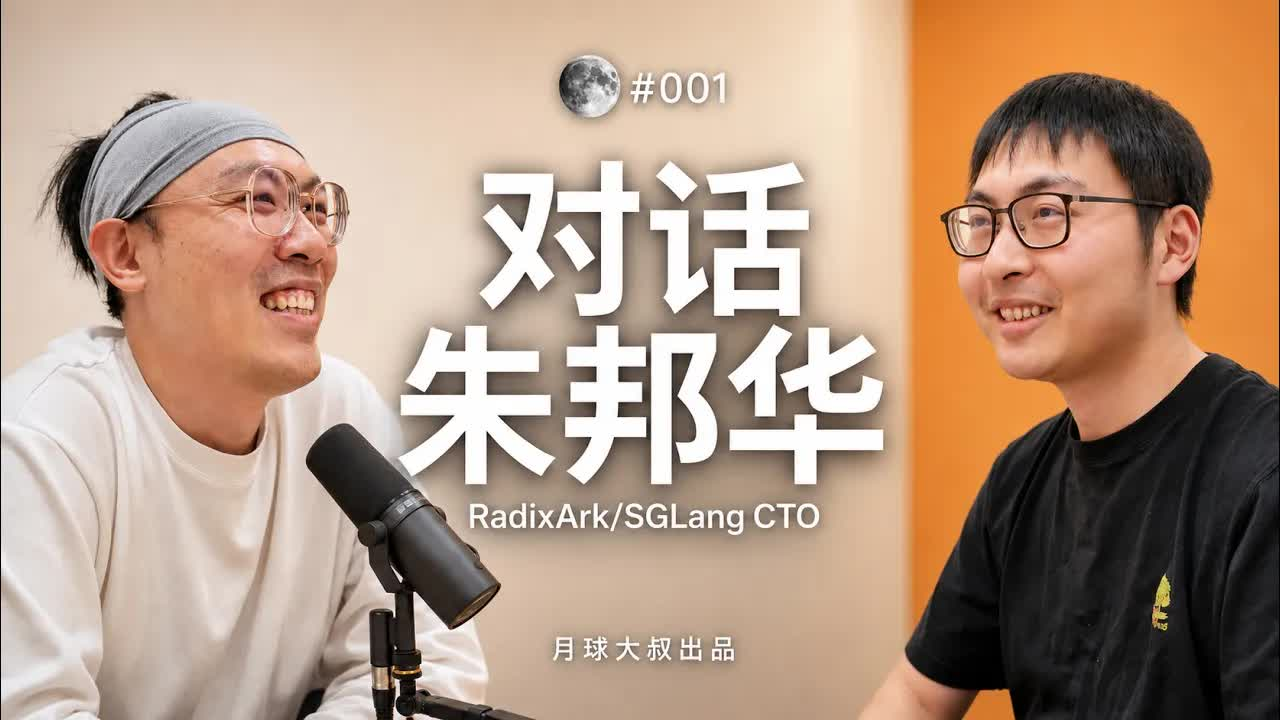
\includegraphics[width=.86\linewidth,height=.27\textheight,keepaspectratio]{cover.jpg}
\par\vspace{6mm}{\small 原节目：朱邦华: SGLang，强化学习，英伟达收购，二次创业，清华，伯克利，LMSYS，Chatbot Arena，善于放弃\par}
\vspace{4mm}主播：月球大叔\par
{\small 朱邦华\par}
\vfill 发布：2026-05-18\par
整理：2026-10-25\quad 正文：Gemini Argon\quad 配图与编校：Codex\par
\vspace{4mm}\url{https://www.youtube.com/watch?v=VoAaX02cHFE}
\end{titlepage}
\begingroup\small\setlength{\parskip}{0pt}\tableofcontents\endgroup\clearpage
\section*{导读}\addcontentsline{toc}{section}{导读}
当大语言模型从对话走向代码编写、工具调用和多步任务执行，决定系统上限的不再只是单次模型调用，而是推理服务、强化学习训练与可执行环境之间的协同。本讲义整理自朱邦华的深度访谈，围绕他从机器学习理论转向大模型后训练与底层基础设施的经历展开。全书沿着技术问题的递进组织内容：首先解析推理服务与强化学习如何通过任务数据形成反馈闭环，说明 SGLang 与 Miles 的定位及新模型适配压力；随后深入强化学习算法内部，对比偏好反馈与可验证奖励的分工，拆解 PPO 训练中的价值网络预热经验；接着将视野扩展到多容器沙箱执行与千卡、万卡分布式训练系统；在此基础上回顾跨学科探索如何塑造研究判断力，展望预训练、同策略蒸馏、持续学习与多模态演进，并探讨开源社区与商业项目的互动、评测标准演进以及智能体时代的技术品味与路径选择。
\needspace{8\baselineskip}\section{从模型能力到推理与训练的闭环}
当大语言模型从通用的聊天演示走向真实的企业业务时，单靠直接调用现成模型往往难以满足复杂任务的成本与准确率要求。本章从朱邦华联合创立的 RadixArk 出发，梳理预训练、后训练与推理服务三个阶段的技术分工，解释真实推理产生的数据如何反哺强化学习训练，并结合 SGLang 的开源演进与新模型首日适配，说明模型架构与底层基础设施为何必须协同演进。
\needspace{6\baselineskip}\subsection{RadixArk 为谁建设基础设施}
在大语言模型（Large Language Model, LLM，基于大规模语料训练、通过预测下一个词元来生成内容或执行指令的神经网络）的应用中，许多团队最初只是直接调用现成模型。随着业务深入，企业需要将模型稳定部署到生产环境中，并根据自身任务调整模型参数，这依赖人工智能基础设施（AI Infrastructure，简称 AI Infra，负责管理算力调度、分布式训练与推理服务的底层软件系统）。在 00:00:40–00:05:14 的访谈中，朱邦华介绍自己毕业后先联合创立了聚焦企业智能体与后训练的 Nexusflow AI，2025 年公司被英伟达收购后担任 NeMo-RL 技术负责人，同年 12 月与长期合作者盛颖共同创立 RadixArk，目标是把前沿人工智能实验室（Frontier AI Lab，拥有大规模算力、持续探索模型能力上限的研发机构）级别的底层系统开放给更多公司与开发者。

要理解 RadixArk 的业务设计，可以先区分大模型生命周期的三个阶段：预训练（Pre-training，在海量文本、代码等广泛数据上训练基础模型，使其掌握语言规律与基础知识）、后训练（Post-training，在预训练模型基础上，通过监督微调或强化学习等方法，使模型对齐人类意图或提升特定任务表现）以及推理（Inference，运行训练好的模型处理在线请求或离线批量任务以生成输出的过程）。在访谈口述中，朱邦华常把业务重点所在的后训练简称为强化学习（Reinforcement Learning, RL，让模型在与环境交互中根据奖励信号调整策略的训练方法）；从完整流程来看，后训练包含监督微调、强化学习等多个环节。

为什么一家基础设施公司要同时布局推理与强化学习训练？朱邦华从团队对不同阶段需求广度的判断给出了原因。从头开展预训练需要投入高昂的算力与资金，有能力且有必要自己做预训练的机构不多；相比之下，后训练的成本更低，企业可以基于开源模型权重，针对自己关心的特定任务或智能体场景做定向强化；而推理则是覆盖面最广的需求，因为任何团队只要在实际场景中使用人工智能，都需要通过推理引擎与模型交互。因此，按他们对需求范围的判断，呈现出“预训练小于后训练、后训练小于推理”的梯度。

围绕这一需求梯度，RadixArk 形成了明确的产品分工：在推理侧维护并推进开源推理框架 SGLang（服务于大语言模型与多模态模型的高效推理系统），在训练侧开发开源强化学习框架 Miles，未来还可能进一步向预训练基础设施延伸。按照节目披露，这两个开源项目已经与北美的谷歌、微软、甲骨文、英伟达、AMD 以及国内的阿里、腾讯、字节跳动等企业开展了深度合作。

\needspace{6\baselineskip}\subsection{从真实使用回到任务训练}
随着开源模型能力提升，企业面临的使用场景不再局限于单轮问答，而是扩展到复杂的智能体任务（Agentic Task，需要模型拆解目标、调用外部工具并在多轮交互中完成具体工作的任务）。通用开源模型能否直接满足特定业务规则与工具调用要求，需要结合具体业务的质量门槛与成本预算来评估。

当现有模型表现达不到业务要求时，企业就有动力探索“推理产生数据、数据反哺后训练”的闭环。当企业在生产环境中高频调用模型进行推理时，系统会沉淀下大量真实的交互轨迹。朱邦华认为，这些私有的垂直行业数据（Private Vertical Data，特定行业或企业内部沉淀的业务流程与交互记录）对强化学习很有价值。不过，原始交互记录并不会自动变成训练提升，必须结合具体任务设计合适的环境反馈或奖励信号，经过筛选和整理后才能用于强化学习。从降本增效的角度看，当通用模型达不到任务标准且内部具备可用反馈数据时，先利用这些数据对模型做后训练、达到更满意的状态后再部署推理，是一条值得投入的路径。

朱邦华在节目中举编程工具公司 Cursor 为例来说明这种做法：团队会选用国内的 Kimi 模型，针对 Cursor 内部的智能体相关能力做进一步后训练，然后再投入推理服务。在他的构想中，推理引擎承接业务流量并记录交互轨迹，强化学习框架利用整理后的任务反馈更新私有模型，更新后的模型再回到推理引擎提供服务，从而将训练与推理连接起来。

从商业落地的节奏来看，目前最直接、规模最大的商业需求仍集中在推理侧，而面向智能体的后训练还处于起步阶段。朱邦华判断，自己动手做后训练的需求可能会经历三层扩散：最先发生在前沿实验室，接着传导至新兴人工智能实验室（Neo Labs，专注探索新一代模型架构或训练范式的初创研究机构）以及像 Cursor 这样的人工智能原生应用公司，再往后逐步延伸到离人工智能稍远的传统企业乃至财富 500 强公司。当传统企业意识到自身业务所需的模型能力超过了现有通用模型提供的水平时，就可能选择自己开展一部分后训练，再将模型投入推理。

\needspace{6\baselineskip}\subsection{SGLang 如何在已有生态中找到位置}
这套训练与推理闭环的底座之一是开源推理框架 SGLang，但朱邦华在加入 RadixArk 之前并不是 SGLang 社区的直接参与者。在 00:08:00–00:16:14 的回顾中，他提到自己读博前四年主要研究机器学习理论、统计学与强化学习理论，直到 2022 年底试用 ChatGPT（GPT-3.5）时，看到一个基于下一词元预测（Next Token Prediction，根据前文词元序列计算下一个词元概率分布的自回归建模方式）的模型能写出简单的算法题代码，才决定转向大语言模型方向。当时他的博士导师迈克尔·乔丹（Michael I. Jordan）从统计学角度提出质疑，认为这只是下一词元预测问题；而朱邦华审视当时的基于人类反馈的强化学习（Reinforcement Learning from Human Feedback, RLHF，利用人类偏好数据训练奖励模型并指导语言模型更新的后训练方法），发现其算法设计还比较粗糙、临时（Ad Hoc），却已经能让模型自然地与人交流。他由此判断，如果后续继续扩大模型参数、数据量与测试时思考长度，并改进后训练算法，模型能力的提升空间会很大。

决定转向后，朱邦华主动发邮件联系了两拨研究者：一拨是伯克利师兄、OpenAI 联合创始人约翰·舒尔曼（John Schulman），双方围绕强化学习算法设计、低秩自适应（Low-Rank Adaptation, LoRA，通过训练低秩矩阵以较少参数量微调大模型的方法）及系统问题展开了交流；另一拨则是当时发表了早期推理系统论文 FlexGen 的盛颖与伯克利同学郑连民。FlexGen 是一套面向受限硬件的推理系统，通过在 GPU、CPU 内存与磁盘之间做分层卸载和调度来运行大模型。这次联系促成了三人的长期合作，盛颖与郑连民随后共同发起了非营利开源研究组织 LMSYS，陆续推出了基于 LLaMA 权重的早期开源对话微调模型 Vicuna（在 Hugging Face 平台上获得千万级下载），以及让用户盲测对比两个模型回答并投票排名的评测平台 Chatbot Arena（后发展为独立公司 LM Arena，节目中提到其估值约 15 亿美元）。

当盛颖与郑连民进一步启动 SGLang 项目时，开源社区里其实已经有了另一个非常流行且成熟度很高的推理引擎 vLLM，并且已经先行发展了近一年时间。朱邦华坦言，自己最初并不看好 SGLang，因为他当时的直觉是：在一个细分领域已经存在优秀开源软件的情况下，再做一个定位高度接近的推理引擎，很难说服用户迁移。因此，那段时间他主要精力放在与导师共同创立的第一家公司 Nexusflow AI 上，基本没有参与 SGLang 的开发。

然而随后一两年的发展改变了他最初的判断。SGLang 的实际采用率持续上升，社区也日益活跃。正如他在后文回顾时所总结的，当推理引擎从第一性原理出发把速度、稳定性和模型支持面做好，并尽早与强化学习训练深度集成时，用户就会选择它。看到社区生态逐渐成熟，且团队希望从推理向包含训练在内的前沿基础设施拓展，这与他在强化学习系统上的背景相契合，最终促成了他加入并联合创立 RadixArk。

\needspace{6\baselineskip}\subsection{新模型为什么需要系统共同演进}
为什么推理与训练基础设施需要随着新模型持续演进？这要从新模型在交互模态与网络架构上的变化说起。在 00:17:31–00:24:23 的讨论中，朱邦华谈到了约翰·舒尔曼参与创立的 Thinking Machines Lab 所展示的实时语音交互模型（Interaction Model）。这类面向多模态或全模态的模型（Omni Model，能够接收并生成语音、文本等多种模态信息的模型）直接以语音作为输入和输出。根据朱邦华观看演示视频与技术博客后的理解（他当时尚未亲自试用），该模型在多轮对话中知道什么时候等待用户、什么时候回话。这种多轮语音交互形式，使得数据准备流水线（Data Pipeline）、词元（Token）设计以及底层系统对全模态模型的支持都面临不同于纯文本模型的新挑战。

除了多模态交互，模型架构的创新同样会给底层系统带来适配压力。SGLang 社区追求在新模型发布首日（Day-1）提供支持，这需要核心开发者（Core-dev）投入大量工程精力。朱邦华以团队支持 DeepSeek V4 相关项目为例说明：由于该模型在架构上做了许多创新，团队在做推理与训练基础设施时需要针对其架构特点做新的改动与优化，其中包括面向前缀缓存（Prefix Cache，缓存多轮对话或共享提示词的前缀计算结果以减少重复计算的机制）的 ShadowRadix，以及面向稀疏注意力（Sparse Attention，只对部分词元计算注意力以降低长序列计算开销的机制）的 HiSparse 等优化。当时仅支持这一项目就投入了约一半核心开发者乃至公司近半数人员的大部分精力，使最终交付的运行性能相比最初拿到模型时获得了大幅改善。

在与中美两国大模型团队合作的过程中，朱邦华也谈到了他个人体验到的风格差异：国内团队的基础设施工程水平很高，写代码速度快、可靠性强，一旦明确了方向，把系统“从 1 做到 100”的执行力很突出；而美国团队在“从 0 到 1”的探索上往往更天马行空，愿意允许研究员尝试各种新奇想法，虽然许多尝试未必成功，但跑通的想法就有可能创造出新的方向。

至于外界关心的开源与闭源模型差距，朱邦华在 2026 年 5 月的访谈中给出了他个人的大致估计：如果拿中国的开源模型与美国的闭源模型相比，差距大约在 6 个月；如果拿美国的开源模型（例如他曾参与过的英伟达 Nemotron 系列，当时仍在快速追赶）与美国的闭源模型相比，差距接近一年。他分析认为，国内开源模型在常规基础设施上做得相当扎实，受限更多在于数据，尤其是国内团队在复杂强化学习交互环境（RL Environment，供智能体执行工具调用、代码运行并获取反馈信号的系统）上的投入相对较少，而美国前沿实验室正持续投资构建更复杂的智能体强化学习环境。这一环节也正是后续章节讨论强化学习算法与环境系统的切入点。

\begin{knowledgebox}{大模型生命周期的三阶段与算力需求梯度}
理解 AI 基础设施的业务与技术逻辑，可以区分三个阶段：
\begin{enumerate}
\item 预训练（Pre-training）：在海量文本、代码等广泛语料上从头训练基础模型，获取通用表征与基础知识。算力与资金门槛高，仅有少数机构直接开展。
\item 后训练（Post-training）：基于预训练权重，利用监督微调（SFT）或强化学习（RL）提升模型在特定任务上的表现或对齐人类偏好。成本低于预训练，适合结合业务反馈数据定向优化模型。
\item 推理（Inference）：运行训练好的模型处理在线交互或批量任务。所有使用 AI 的场景都离不开推理，因此其应用覆盖面与直接商业需求最广。
\end{enumerate}
\end{knowledgebox}
\begin{warningbox}{何时需要从直接推理走向后训练闭环}
是否对开源模型做后训练，取决于业务任务门槛与数据条件。如果通用模型已能满足准确率与成本要求，直接部署推理即可；但面对复杂的企业级智能体任务（Agentic Task），当现有模型能力达不到业务标准，且线上推理沉淀的私有垂直数据能够整理出有效的任务评估与奖励信号时，通过后训练定向强化模型再重新部署推理，就能形成兼顾任务效果与长期成本的工程闭环。
\end{warningbox}
\begin{table}[H]\centering\small
\caption{大模型研发与服务核心环节及 RadixArk 对应布局}
\begin{tabular}{>{\raggedright\arraybackslash}p{\dimexpr(\linewidth-8\tabcolsep)/4\relax}>{\raggedright\arraybackslash}p{\dimexpr(\linewidth-8\tabcolsep)/4\relax}>{\raggedright\arraybackslash}p{\dimexpr(\linewidth-8\tabcolsep)/4\relax}>{\raggedright\arraybackslash}p{\dimexpr(\linewidth-8\tabcolsep)/4\relax}}
\toprule
生命周期阶段 & 核心解决的问题 & 关键机制与系统挑战 & 访谈中的工具或案例\\\midrule
预训练 (Pre-training) & 从海量原始数据中学习通用表征与基础知识 & 超大规模算力集群调度、万亿参数容错与高成本控制 & 仅少数前沿实验室开展，RadixArk 的远期拓展方向\\[4pt]
后训练 (Post-training / RL) & 将基础模型定向对齐到特定任务、工具调用或人类偏好 & 利用私有垂直数据与强化学习环境交互更新模型权重 & 开源强化学习框架 Miles；Cursor 基于 Kimi 做内部强化\\[4pt]
推理服务 (Inference) & 低延迟、高吞吐地响应线上请求并生成多模态或文本输出 & 前缀缓存（如 ShadowRadix）、稀疏注意力优化（如 HiSparse）与算子调度 & 开源推理框架 SGLang、vLLM、早期研究 FlexGen\\[4pt]
模型评测与数据回流 & 检验模型真实交互质量，沉淀线上轨迹反哺下一轮训练 & 盲测偏好投票、复杂智能体环境验证与私有数据闭环 & Chatbot Arena (LM Arena)、企业线上推理日志收集\\[4pt]
\bottomrule\end{tabular}\end{table}
前文指出，当企业面对复杂的智能体任务时，直接调用通用模型未必能满足内部业务规范。为了让推理服务与强化学习后训练相互促进，需要将线上调用与模型更新连接成闭环，下图展示了这一流程的关键环节。
\begin{figure}[H]\centering
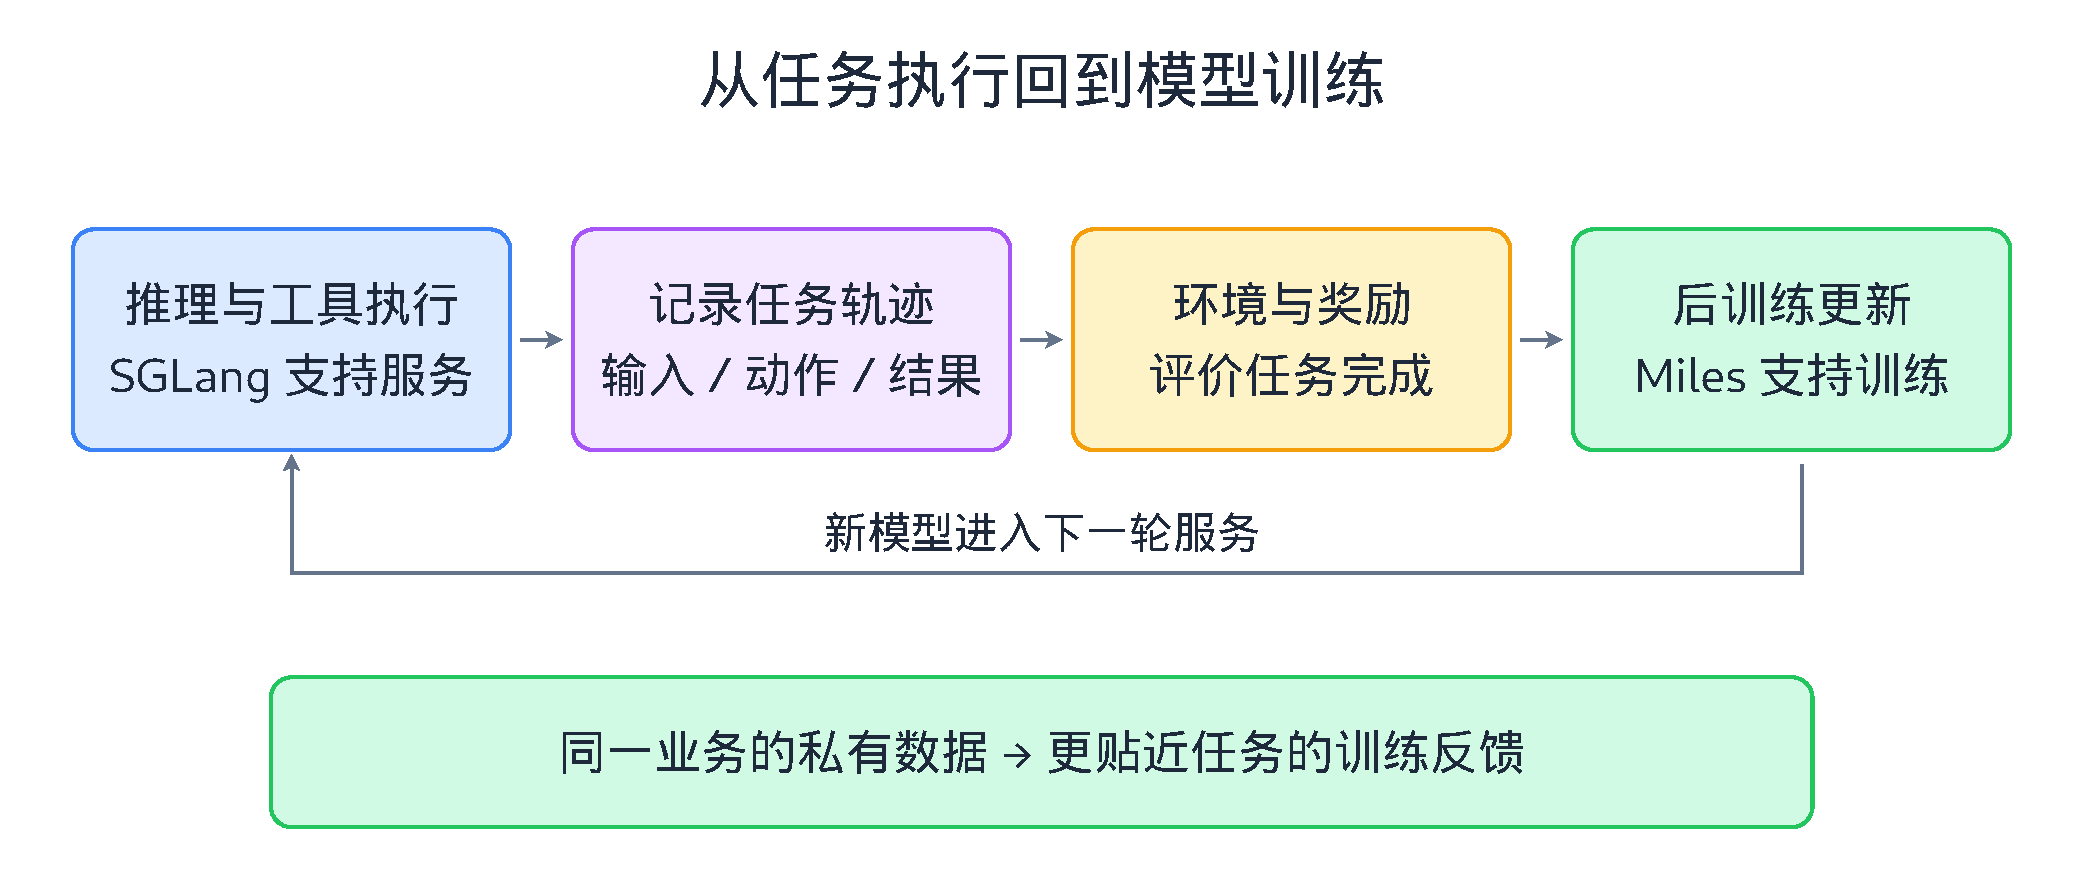
\includegraphics[width=\linewidth,height=.68\textheight,keepaspectratio]{assets/training-inference-loop.pdf}
\caption{从任务执行回到模型训练；依据节目口述整理（00:02:52–00:07:45）}
\end{figure}
\begin{knowledgebox}{读图：从模型能力到推理与训练的闭环}
图上方由四个从左到右依次以箭头相连的方框组成：最左侧是“推理与工具执行（SGLang 支持服务）”，指向“记录任务轨迹（输入／动作／结果）”，再指向“环境与奖励（评价任务完成）”，最后到达最右侧的“后训练更新（Miles 支持训练）”。一条回流箭头从“后训练更新”底部引出，标注“新模型进入下一轮服务”并指回最左侧方框；图下方横框总结为“同一业务的私有数据 \ensuremath{\rightarrow} 更贴近任务的训练反馈”。
\end{knowledgebox}
这表明原始交互轨迹必须经过环境与奖励环节的任务完成度评价，才能转化为后训练更新的有效信号，这也引出了下一章关于强化学习如何利用反馈更新权重的具体机制。
\needspace{6\baselineskip}\subsection{本章小结}
\begin{enumerate}
\item 按团队对市场需求广度的判断，大模型基础设施呈现“预训练 < 后训练 < 推理”的梯度，RadixArk 通过开源推理框架 SGLang 与强化学习框架 Miles 覆盖从推理服务到模型后训练的链路。
\item 在复杂智能体场景中，当通用模型未达业务要求且企业具备经过整理的有效反馈数据时，利用线上推理沉淀的私有数据开展后训练并重新部署，能够构成“推理—训练”的正向闭环。
\item 无论是实时语音等多模态交互，还是像 DeepSeek V4 这样的新架构设计，都会对数据流水线、前缀缓存（如 ShadowRadix）与稀疏注意力（如 HiSparse）提出新的适配要求，推动推理与训练系统随模型共同演进。
\end{enumerate}
\needspace{8\baselineskip}\section{强化学习怎样把反馈变成模型更新}
明确了训练与推理相互促进的业务闭环后，接下来的核心技术问题是：当系统收集到人类偏好或环境执行结果时，强化学习究竟如何将这些反馈转化为模型参数的更新？本章回到朱邦华在 Nexusflow AI 与 Starling 模型上的早期实践，剖析比较排序数据与不同奖励范式的分工，解释近端策略优化在工程实现中为何容易崩溃，并演示如何通过预热价值网络完成稳定的策略更新。
\needspace{6\baselineskip}\subsection{Nexusflow、Starling 与反馈数据}
在 2023 年初大语言模型兴起时，开源社区改善模型表现常见的方式是监督微调（Supervised Fine-Tuning, SFT，用“指令—示范回答”配对数据训练模型，使其学习给定格式与行为）。但仅靠模仿示范文本，模型不易区分不同回答的优劣。在 00:27:25–00:29:24 的访谈中，朱邦华回顾了自己转向大模型后与博士导师共同创立 Nexusflow AI 的契机：团队当时推出了一个 70 亿参数（7B）的开源模型 Starling，并在盲测对比榜单 Chatbot Arena 上取得了很高的分数。

要通过强化学习提升模型对话质量，第一步是解决反馈数据的匮乏。当时的开源社区非常缺乏多回答比较数据（Multi-response Comparison Data，针对同一个提示词生成多个不同回答，并对这些回答做优劣排序的数据集）。为了构建这套数据与训练流水线，团队采用了基于人工智能反馈的强化学习（Reinforcement Learning from AI Feedback, RLAIF，利用强大的 AI 模型代替人工，对同一问题的多个候选回答进行打分或排序，以此训练奖励模型并优化语言模型的后训练方法）。

虽然调通 7B 模型本身的训练用了不到一个月，但前期准备并开源这套多回答比较与排序数据集耗费了团队不少精力。在这类强化学习框架中，有两个基础组件：被训练的大语言模型本身称为策略网络（Policy，记作 \(\pi_\theta\)，负责根据输入上下文生成词元序列的概率分布），而利用排序数据训练出来的打分模型则称为奖励模型（Reward Model，把输入问题和候选回答映射为标量分数，用来评估回答质量的辅助模型）。

当 Starling 验证了通过 RLAIF 可以改善模型的对话交流表现后，朱邦华认为同样的思路可以迁移到企业智能体上。因此，Nexusflow AI 随后将强化学习扩展到函数调用（Function Calling，模型按约定格式输出工具名称与参数以触发外部操作的能力）以及数学、代码等可验证任务上，将训练规模扩展到 30B 和 70B 模型，并构建了面向函数调用的评测基准与合成数据生成流水线（Synthetic Data Generation Pipeline，利用模型与规则批量构造训练数据的流程），其中一些后训练技巧也在与 LLaMA 团队交流后被用于 LLaMA 2 与 LLaMA 3 的后训练中。

\needspace{6\baselineskip}\subsection{RLHF、RLAIF 与 RLVR 的分工}
为什么后训练阶段既需要偏好打分，又需要针对代码和数学的客观检验？在 00:35:58–00:39:18 的讨论中，朱邦华对比了不同强化学习范式的侧重点。首先是 RLHF，它的主要思路是让模型生成的内容更符合人类的交流习惯与偏好。具体做法是对同一个提示词生成多个回答，由人工标注哪些回答更好、哪些更差，据此训练出一个奖励模型，再用该奖励模型给出的信号指导语言模型训练。经过这一训练，模型在回答问题时能够提供更详尽、更自然的表达；同时，RLHF 也常作为模型训练的最后阶段之一，利用奖励模型信号辅助实现人类价值观对齐（Alignment）与安全目标。

与依赖主观偏好打分的 RLHF 或 RLAIF 不同，可验证奖励强化学习（Reinforcement Learning with Verifiable Rewards, RLVR，直接使用外部规则、编译器或标准答案对模型输出做客观对错检验并提供奖励信号的训练方法）专门针对能够被明确验证真伪的领域。例如求解一道数学题、编写一段需要通过单元测试的代码，或者在智能体环境中完成一个特定操作目标。在这些场景下，系统不需要再训练一个神经网络去猜测人类喜不喜欢，而是直接计算数学结果是否正确、代码能否跑通，从而给出高度客观的奖励信号。

正是 RLVR 的进展，改变了许多团队对强化学习必要性的认识。朱邦华提到，早期不少人认为只要拿强模型的输出做监督微调（SFT）就够了，未必需要做强化学习；直到 DeepSeek 的相关发布证明，开展大规模 RLVR 训练能够提升模型的推理能力，甚至直接从预训练检查点（Pretrained Checkpoint，完成预训练阶段保存下来的模型权重）启动 RLVR 也能跑通（这一直接跳过 SFT、从基础模型启动大规模强化学习的实验对应于 DeepSeek-R1-Zero）。朱邦华认为，这一进展让包括英伟达在内的产业界更加重视强化学习，也成为推动 Nexusflow AI 被收购的契机之一。

在实际研发流程中，RLHF 与 RLVR 并非相互替代，而是可以组合使用。RLVR 借助客观验证器，在数学、编程以及工具调用等可验证任务上提升模型的解题与执行表现；而 RLHF（及 RLAIF）则利用奖励模型处理难以用固定规则写死的人类偏好、表达风格与对齐要求，二者共同服务于后训练的不同目标。

\needspace{6\baselineskip}\subsection{PPO 为什么会在实现中失效}
拿到奖励信号后，接下来的问题是如何用算法更新策略网络。在 00:29:24–00:31:28 的访谈中，朱邦华回忆道，尽管 OpenAI 很早就表示使用近端策略优化（Proximal Policy Optimization, PPO，一种通过裁剪目标限制单次策略更新幅度、以减轻训练不稳定倾向的演员-评论家算法）取得了良好效果，但 2023 年许多复现尝试却未能跑通。由于调通 PPO 门槛较高，不少团队转而采用直接偏好优化（Direct Preference Optimization, DPO，一种绕过显式奖励模型建模与在线强化学习采样，直接依据偏好回答对与参考策略优化对比目标的算法）。

为什么许多人当时觉得 PPO 不起作用？这与 PPO 涉及的组件和估计过程有关。除了生成回答的策略网络（Policy）和提供分数的奖励模型外，PPO 还需要训练一个价值网络（Critic，也称 Value Function，记作 \(V_\phi(s_t)\)，其中 \(\phi\) 为价值网络的参数，用于估计在时间步 \(t\) 的上下文状态 \(s_t\) 下后续期望获得的总回报）。在训练中，若用一步时序差分（TD）残差 \(\delta_t\) 来说明优势估计的基本形式，可写为：
\[
\delta_t = r_t + \gamma V_\phi(s_{t+1}) - V_\phi(s_t)
\]

其中 \(r_t\) 是时间步 \(t\) 获得的即时奖励，\(\gamma\) 是衡量未来奖励权重的折扣因子（Discount Factor）。在实际 PPO 实现中，通常还会将多步残差 \(\delta_t\) 组合为广义优势估计（GAE）来计算优势值 \(A_t\)，用以衡量当前动作相比状态平均水平的好坏。优势估计与学习率、裁剪范围等因素共同影响策略参数的更新：若优势估计为正，算法倾向于提高该动作的生成概率；反之则降低其概率。

从这个过程可以看出，PPO 调通难度高的一个重要原因在于训练基础设施（Infra）的实现细节。朱邦华指出，强化学习的系统实现未必是花哨的概念，但如果在分布式采样、奖励处理、折扣因子设计或梯度计算等环节不够仔细，就容易留下隐蔽的实现瑕疵（暗坑），导致计算出的更新信号失真，进而让人得出相反或错误的结论。此外，PPO 涉及价值网络训练方式、折扣因子及各类超参数（Hyperparameter，训练前设定的配置参数），调参空间很大。

针对 PPO、DPO 以及后来兴起的群组相对策略优化（Group Relative Policy Optimization, GRPO，无需单独训练价值网络 Critic，而是对同一问题采样一组回答，利用组内奖励的相对统计量计算优势的强化学习算法），朱邦华给出了基于实验观察的视角：2023 年他认为只要把工程实现和调参细节做好，PPO 的上限很高，Starling 的训练结果也支持了这一点；而随着后续算法发展，像 GRPO 这样省去独立价值网络、结构更简化的算法逐渐普及，使用 GRPO 的人越来越多，做传统 PPO 的人相应减少。正如他在后文所强调的，面对不同算法路线，不能仅凭个人偏好把某种方法说死，结论需要建立在严谨的实验观察之上。

\needspace{6\baselineskip}\subsection{先预热 critic，再更新 policy}
在维度很高、无法靠穷举搜索遍历所有超参数的强化学习训练中，研究者是如何把 PPO 调通的？在 00:31:28–00:34:05 的对话中，朱邦华将其概括为“依靠直觉（Intuition）选择方向—通过实验验证部分假设—再提出新直觉”的探索过程。为了具体说明这种调参经验，他举了训练价值网络（Critic）时的一个例子。

在他们启动 PPO 训练的设置中，策略网络（Policy）已经是具备生成能力的语言模型，而价值网络（Critic）可能是随机初始化的，或者是从奖励模型（Reward Model）初始化后新加了一个输出头（Head）。在训练刚起步时，这个尚未校准的价值网络初期损失函数（Loss Function，衡量预测值与目标值差距的指标）往往很高，在他举的例子里可能从 2、3 这样的个位数开始，而训练稳定后的损失可能在零点零几的量级，需要训练一段时间才会下降。

如果在价值网络误差还很大的最初阶段，就直接用它去同步优化策略网络（语言模型本身），由于价值网络给出的更新方向和梯度不够准确，就会使语言模型的权重发生很大偏移。在朱邦华描述的训练经历中，如果不处理这一问题，开局阶段的不良更新就可能把模型破坏掉，导致后续训练难以救回。

针对这一现象，他介绍的实用做法是“先预热 Critic，再更新 Policy”。具体来说，在开启完整的 PPO 联合训练之前，先针对当前固定的策略用一批数据单独训练价值网络（即 Critic Warm-up）一段时间，让它的损失函数降到较低且相对收敛的水平；等价值网络能够较好地拟合当前策略的回报后，再用它来初始化并进入正式的 PPO 训练。朱邦华提到，这种分步预热是他们在调参中摸索出的实践技巧，具体预热时长与设置取决于实际任务。

\begin{importantbox}{何时先预热价值网络（Critic Warm-up）}
在包含价值网络的 PPO 训练中，为什么有时需要先预热 Critic 再联合更新 Policy？
\begin{enumerate}
\item 初始状态差异：当 Policy 已具备语言生成能力，而随机初始化或新加输出头的 Critic 尚未适应当前策略时，初期的价值预测损失可能较高。
\item 优势估计偏差：由一步残差 \(\delta_t = r_t + \gamma V_\phi(s_{t+1}) - V_\phi(s_t)\) 可见，不准确的价值估计 \(V_\phi\) 会导致优势估计偏差，进而影响策略梯度的方向。
\item 策略偏移风险：若在初期直接用偏差较大的梯度大幅更新 Policy，可能破坏语言模型原有的生成表现。
\item 实践做法：先针对当前策略的数据单独训练 Critic 使其损失下降并趋于收敛，再进入 Policy 与 Critic 的联合训练。
\end{enumerate}
\end{importantbox}
\begin{warningbox}{区分算法潜力与系统实现细节}
2023 年许多团队复现 PPO 未果后，容易认为 PPO 本身不适合大模型。实际上，强化学习对底层基础设施（Infra）的实现细节很敏感：从奖励处理、折扣因子设置到 Critic 预热，任何一处实现瑕疵都可能导致更新信号失真。DPO、PPO 与后来的 GRPO 各有不同的工程复杂度与适用场景，需要结合具体的系统实现质量与实验观察来评估，而不宜把某种算法绝对说死。
\end{warningbox}
\begin{table}[H]\centering\small
\caption{大模型后训练核心强化学习范式与优化算法对比}
\begin{tabular}{>{\raggedright\arraybackslash}p{\dimexpr(\linewidth-8\tabcolsep)/4\relax}>{\raggedright\arraybackslash}p{\dimexpr(\linewidth-8\tabcolsep)/4\relax}>{\raggedright\arraybackslash}p{\dimexpr(\linewidth-8\tabcolsep)/4\relax}>{\raggedright\arraybackslash}p{\dimexpr(\linewidth-8\tabcolsep)/4\relax}}
\toprule
技术概念 & 核心解决的问题 & 反馈来源或优势计算机制 & 工程实践中的定位与特点\\\midrule
RLHF / RLAIF & 让模型回答自然得体，对齐人类偏好与安全价值观 & 人工或强 AI 对多回答排序，训练奖励模型（Reward Model）输出连续分数 & Starling 借助 RLAIF 刷榜 Arena；常作为模型对齐与安全的最后训练阶段\\[4pt]
RLVR (可验证奖励强化学习) & 提升数学、代码及复杂智能体任务的客观推理与执行准确率 & 不依赖主观偏好模型，直接由编译器、数学答案或环境验证器给出客观奖励 & 如 DeepSeek-R1-Zero 直接从预训练检查点开展大规模强化学习，提升推理表现\\[4pt]
PPO (近端策略优化) & 在限制单步更新幅度的前提下，利用在线采样稳定提升策略表现 & 需同时维护 Policy 与 Critic，通过价值估计计算优势函数并裁剪更新步长 & 调通后上限很高，但超参数多、对实现细节敏感，通常需配合 Critic 预热等技巧\\[4pt]
DPO / GRPO & 降低 PPO 维护独立价值网络（Critic）带来的显存开销与调参难度 & DPO 依据偏好对与参考策略优化对比目标；GRPO 通过同一问题组内多个回答的相对奖励计算优势 & 省去 Critic 训练负担，工程链路更简洁，GRPO 在后续推理与智能体训练中广泛普及\\[4pt]
\bottomrule\end{tabular}\end{table}
在理解了 PPO 利用优势估计更新策略的机制后，工程实践中的一个常见难题是训练初期的价值网络尚未校准。朱邦华结合自身调参经历，说明了初始误差如何干扰策略更新，以及如何通过分阶段预热解决这一问题。
\begin{figure}[H]\centering
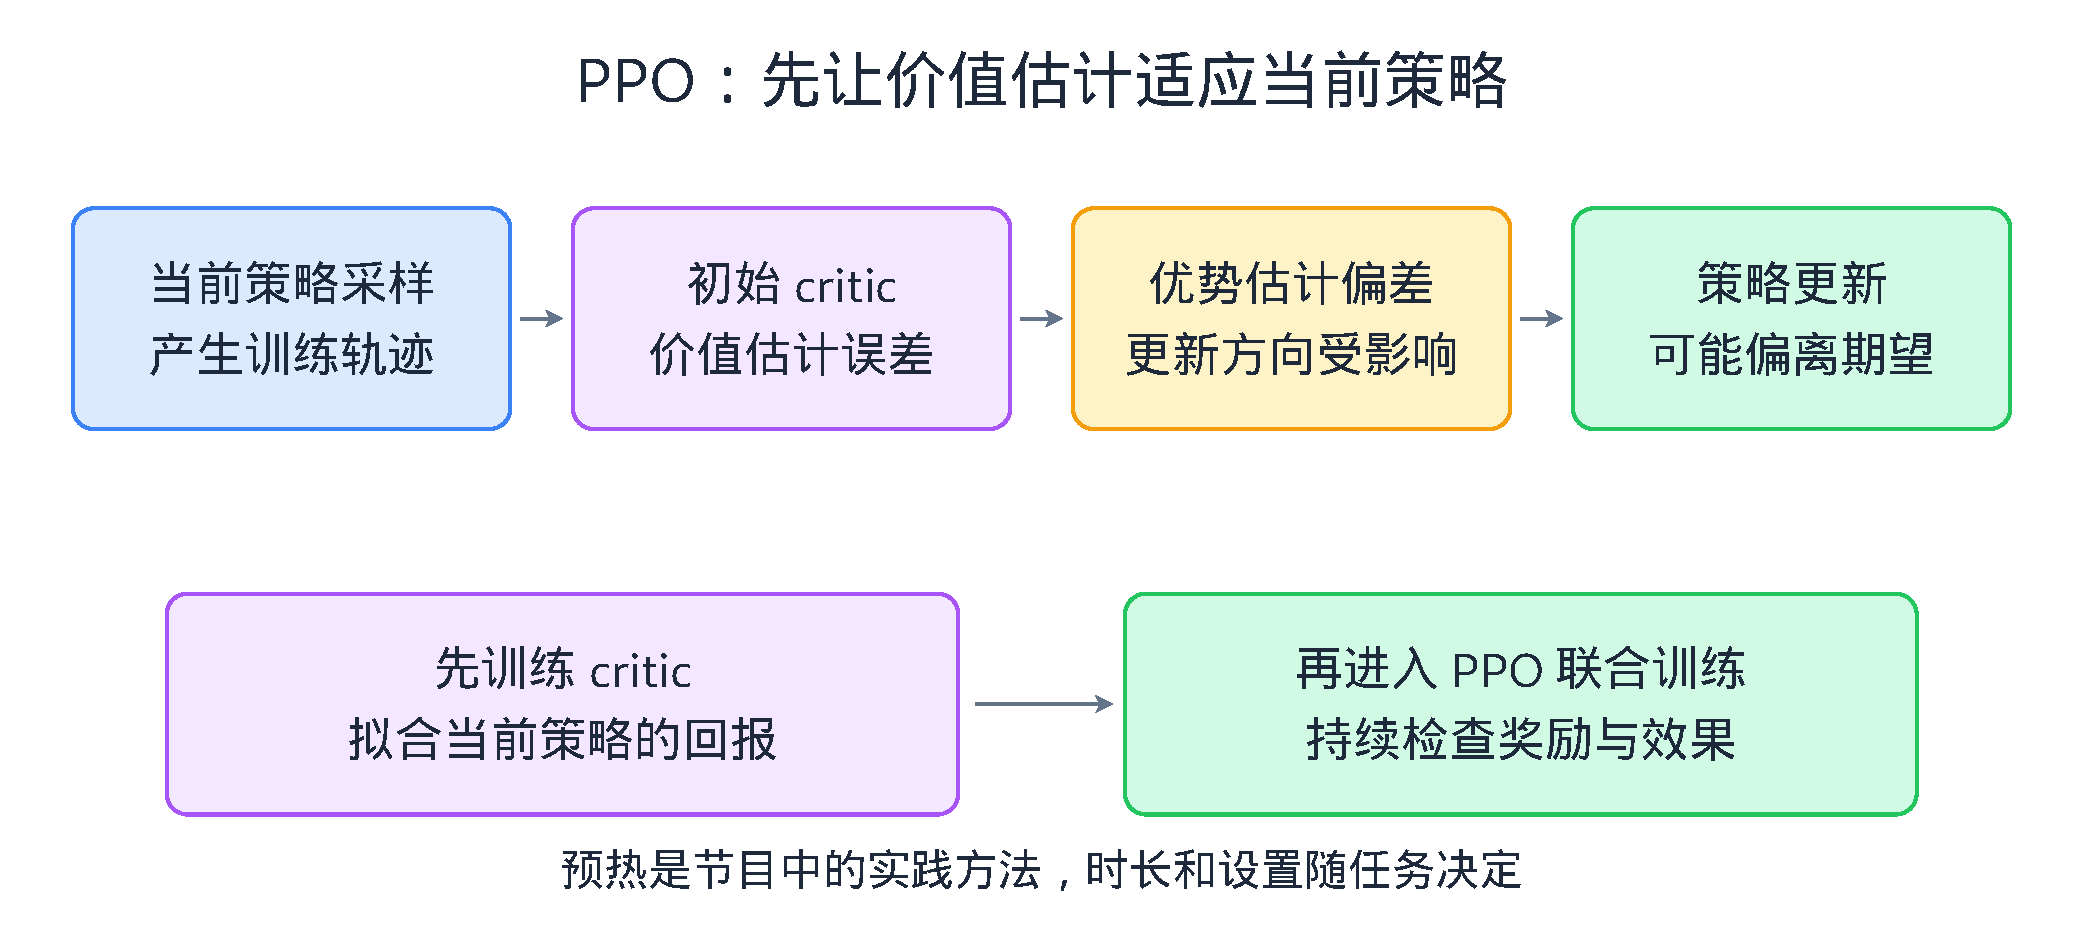
\includegraphics[width=\linewidth,height=.68\textheight,keepaspectratio]{assets/critic-warmup.pdf}
\caption{PPO：先让价值估计适应当前策略；依据节目口述整理（00:29:30–00:33:46）}
\end{figure}
\begin{knowledgebox}{读图：强化学习怎样把反馈变成模型更新}
图形分为上下两行对照。上行四个方框从左到右由箭头连接：“当前策略采样（产生训练轨迹）”指向“初始 critic（价值估计误差）”，再指向“优势估计偏差（更新方向受影响）”，最终指向“策略更新（可能偏离期望）”。下行展示改进做法，左侧宽框“先训练 critic（拟合当前策略的回报）”通过箭头指向右侧宽框“再进入 PPO 联合训练（持续检查奖励与效果）”。底部文字注明：“预热是节目中的实践方法，时长和设置随任务决定”。
\end{knowledgebox}
通过对比上下两条路径可以看到，先让价值网络适应当前策略的回报分布，能够减轻初期优势估计偏差对策略权重的冲击。下一章将进一步从单步算法走向外部执行环境与大规模训练系统。
\needspace{6\baselineskip}\subsection{本章小结}
\begin{enumerate}
\item 强化学习后训练依赖对比反馈数据：Nexusflow 早期的 Starling 模型通过构建多回答比较排序数据与 RLAIF 流水线，提升了模型的对话表现。
\item RLHF/RLAIF 与 RLVR 可以互补配合：前者借助奖励模型学习人类偏好与对齐要求，后者借助代码执行、数学检验等客观验证信号提升模型在可验证任务上的能力。
\item PPO 训练效果受基础设施实现精度与调参细节影响很大；当初始价值网络误差较大时，先预热价值网络（Critic）使其适应当前策略，再联合更新语言模型（Policy），是避免初期不良梯度破坏模型的实用经验。
\end{enumerate}
\needspace{8\baselineskip}\section{从可执行环境到千卡训练系统}
上一章剖析了强化学习在单次策略更新中的算法细节与价值网络预热技巧。然而，当训练目标从静态文本问答转向能够调用工具、编写并执行代码的复杂智能体时，制约模型进化的瓶颈便从算法公式延伸到了底层工程系统。本章将跟随朱邦华从创业公司到英伟达、再到 RadixArk 的实践视角，拆解可执行强化学习环境中的 CPU 调度瓶颈、环境数据与奖励设计的分工，以及算力规模从几十张卡跃升至千卡、万卡级别时面临的分布式系统挑战。
\needspace{6\baselineskip}\subsection{模型等待的可能是 CPU 和工具}
在理解了近端策略优化（PPO）等强化学习算法如何利用奖励信号更新权重后，一个自然的工程问题是：如果我们要训练一个会操作电脑、会写代码或调用外部工具的智能体（Agent），整个训练系统的速度是由什么决定的？在 00:24:23–00:26:21 的讨论中，朱邦华指出，强化学习环境（RL Environment，即智能体在训练时与之交互、执行动作并获取状态反馈与奖励的外部运行系统）是人工智能基础设施中极易被忽视却至关重要的一环。

为什么环境会成为整个大模型训练的瓶颈？在传统的纯文本后训练中，图形处理器（Graphics Processing Unit, GPU，擅长大规模并行矩阵运算的加速芯片）只需要把词元生成出来，交由另一个位于 GPU 上的奖励模型打分即可。但在智能体强化学习中，模型生成的是函数调用（Function Calling）指令或一段待验证的程序代码。此时，系统必须等待外部环境真正把这个函数或代码执行完、返回运行结果后，模型才能继续下一步推理或计算奖励。如果函数调用的响应时延（Latency，单次操作从发出请求到收到结果耗费的时间）无法控制，或者环境支持的并发度（Concurrency，系统同时处理多个独立执行请求的能力）不够高，昂贵的 GPU 集群就会陷入漫长的空转等待。

这也解释了为什么在大模型训练进入智能体阶段后，中央处理器（Central Processing Unit, CPU，负责通用逻辑控制、操作系统调度与工具执行的处理器）的调度能力变得尤为关键。在执行代码（Code Execution）或运行多容器环境（Multi-Docker Environment，利用 Docker 容器技术同时运行多个相互隔离的运行环境）时，进程管理、容器调度与诸多工具执行都依赖 CPU（同时还可能涉及网络、存储或外部服务）。如果 CPU 侧的并发调度跟不上 GPU 采样的速度，整个强化学习训练链路就会受阻于环境执行环节。

基于这一系统洞察，朱邦华在分析当时国内外开源模型与闭源前沿模型（Frontier Model）的差距时提出，国内团队在常规训练与推理基础设施（Infra）上其实做得相当扎实，真正的短板往往在于复杂强化学习环境的数据与投入。前沿实验室要想继续推高模型能力上限，就必须不断投资构建更复杂的智能体强化学习基础设施，并与底层的训练框架做深度适配。

\needspace{6\baselineskip}\subsection{任务环境与奖励设计是两类工作}
既然强化学习环境如此重要，产业界围绕环境构建具体在解决哪些问题？朱邦华指出，硅谷涌现的像 E2B 等强化学习环境相关公司，实际上涵盖了两个层面的工作：一类是构建强化学习环境的底层基础设施（Environment Infra），另一类是专门构建环境中的任务提示词与对应的奖励机制（Task \& Reward Data），并提供给前沿实验室。

这两个层面对应着不同的工程与研究重心：底层环境基础设施关注沙箱如何高并发、低时延地运行；而上层的任务与奖励数据构建，则关注在环境中给模型布置什么任务（Prompt）以及如何评估任务完成度（Reward）。朱邦华认为，对于许多前沿实验室而言，要让已经具备较强基础能力的模型继续进步，一个重要途径就是构建模型当前尚会失败（Fail）的更复杂环境，让模型在这些环境中通过强化学习逐步学会完成目标。

在构建高质量环境的各个环节中，朱邦华把“如何设计奖励（Reward Design）”比作一门艺术问题。如果奖励信号设计得不够合理，模型在复杂环境中就难以获得有效的提升信号。只有把任务环境与奖励机制设计妥当，才能支持模型在复杂任务上持续进步。

此外，当智能体任务从单步工具调用走向像 Claude Code（在终端与代码库中同开发者进行多轮交互、修改代码并运行测试的编程智能体）这样的多轮交互场景时，还面临另一个开放问题：如何在训练环境中模拟一个高质量的人类用户（Simulate a User）。在多轮交互中，用户的反馈与后续指令会影响整个任务轨迹，如何构建逼真的模拟用户并把环境数据做好，是智能体强化学习继续深入的重要方向。

\needspace{6\baselineskip}\subsection{NeMo Gym 如何汇集组织内的数据}
为了具体说明大型科技公司如何组织强化学习环境与数据，我们可以看向朱邦华在 00:41:21–00:43:52 分享的英伟达（NVIDIA）工作经历。2025 年 Nexusflow AI 被收购后，朱邦华加入英伟达担任强化学习框架相关技术负责人，期间他主导并发起了一个内部初期项目——NeMo Gym。这个名字借鉴了强化学习历史上著名的 OpenAI Gym（一套标准化的强化学习环境接口库），旨在解决大型组织内部智能体数据与环境分散的痛点。

在英伟达这样规模庞大的企业里，不同业务部门和研究小组手里其实沉淀了各种各样优秀的想法、内部业务场景以及高质量的数据。如果缺乏统一的平台，这些宝贵的智能体交互数据和环境就会散落在各个团队的孤岛中。NeMo Gym 启动时的核心思路，就是建立一个全公司共享的汇集机制，把各个团队内部想做的智能体任务数据、强化学习环境乃至部分监督微调（SFT）数据全部收集并整合起来，统一用于训练英伟达自家的 Nemotron 系列模型。这个最初由小团队发起的尝试，后来逐渐扩展为整个公司层面的跨部门协作项目。

在理解 NeMo Gym 时，需要区分节目口述中已经完成的部分与团队原本的远期目标。据朱邦华介绍，团队原本的远期目标是将 NeMo Gym 做成更完备的智能体基础设施（Agent Infra），使研究人员在做后训练时只需与 NeMo Gym 交互，由系统收集数据、决定采用怎样的数据组合来训练当前模型，并优化底层智能体基础设施。

而在实际推进中，当时 NeMo Gym 主要完成的是“智能体数据的收集与汇集（Data Collection）”这一部分，尚未实现自动数据配比决策与底层设施自动优化。即便如此，将组织内部多样的强化学习环境与数据汇集起来，已经对 Nemotron 模型的强化学习训练起到了很大帮助。

\needspace{6\baselineskip}\subsection{卡数增长改变了系统问题}
除了汇集环境数据，从初创公司进入英伟达带给朱邦华的另一个明显变化，是从算力紧缺（GPU Poor）变成了算力充裕（GPU Rich）。在早期的 Nexusflow AI 阶段，团队通常只有 2 到 4 个计算节点（Node，包含多张 GPU 的物理服务器；按每节点 8 张 H100 GPU 计算，4 个节点为 32 张卡），在这样的条件下开展了 30B 和 70B 模型的后训练。而当模型参数达到万亿（Trillion）级别、算力规模扩展到千卡甚至万卡级别时，整个基础设施面临的系统问题发生了很大变化。

为什么在几个节点上做训练的经验，不能直接外推（Generalize）到千卡或万卡集群？在 00:44:07–00:46:27 与 01:11:08–01:13:34 的访谈中，朱邦华列举了大规模分布式训练面临的几项核心挑战：
\begin{itemize}
\item 容错与故障恢复（Fault Tolerance）：当集群扩展到千卡、万卡规模时，硬件或节点异常更容易出现，系统需要具备相应的容错机制，在节点失效后能够恢复并接续训练。
\item 正确性与精度匹配（Accuracy Match）：在大规模并行、容错恢复与各类系统优化叠加后，一些原本在小规模实验中未暴露的边缘情况（Corner Case）更容易出现，可能导致训练精度产生偏差；必须验证优化后的系统仍能匹配预期的数值行为与训练结果，避免研究人员因系统偏差得出错误结论。
\item 模型算力利用率（Model FLOPs Utilization, MFU，集群每秒实际完成的模型有效浮点运算次数与硬件理论峰值每秒浮点算力的比值）：规模扩大后，跨节点通信与协同开销增加，维持整个集群较高的 MFU 需要更深入的系统调优。
\end{itemize}

朱邦华谈到，之所以从前沿实验室出来的研究人员受关注，很大程度上是因为“人都是被卡养出来的”——只有亲身接触过大规模集群，才能积累起训练超大模型的系统经验。在算力充裕的条件下，面对高维度的搜索空间，研究人员有时不必对每个细枝末节都做繁琐的消融实验，而是可以结合研究直觉直接启动较大规模的训练运行来探索数据、算法与基础设施的组合（即他在口述中提到的“YOLO run”）。在他个人的观察中，在这种算力环境下，有的本科生因为没有过多思维束缚、敢于尝试，甚至可能比过于谨慎的博士生跑出更好的训练结果。

看到开源社区与前沿实验室在大规模强化学习基础设施上的差距，朱邦华与团队在 RadixArk 推出了开源强化学习框架 Miles。单纯依靠开源社区很难凑齐千卡或万卡集群去反复测试系统可靠性，而通过商业项目合作，团队得以在更大规模的集群上检验系统并回馈社区。根据访谈口述，Miles 框架当时已经历过千卡级别的测试验证，而在万卡级别上，仍需要对容错机制与数据采集调度层（Acquisition Layer）做进一步优化。

\begin{knowledgebox}{强化学习系统的双层架构：沙箱执行层 vs. 任务奖励数据层}
在构建面向智能体（Agent）的强化学习环境时，相关工作可分为两个层面：
\begin{enumerate}
\item 沙箱执行与基础设施层（Environment Infra）：主要解决工具调用与代码执行时的时延（Latency）与并发（Concurrency）瓶颈。多容器环境（Multi-Docker）的进程调度与工具执行依赖 CPU 及相关运行资源，若并发不足或响应过慢，就会阻塞 GPU 采样。
\item 任务构造与奖励设计层（Task \& Reward Data）：主要解决“布置什么任务（Prompt）”与“如何设计奖励（Reward）”。包括构建模型当前尚会失败的复杂环境、设计合理的奖励信号，以及在多轮交互场景中模拟人类用户（Simulate a User）。
\end{enumerate}
\end{knowledgebox}
\begin{warningbox}{为什么小集群经验需要经过千卡、万卡规模验证}
在几个节点（如 32 张 H100）上顺利开展 30B 或 70B 模型的后训练，并不意味着同一套系统经验能直接平移到千卡、万卡或万亿参数模型。当卡数大幅增加时，节点故障与边缘情况（Corner Case）更容易暴露。系统必须在真实规模上检验容错恢复（Fault Tolerance）、计算精度匹配（Accuracy Match）以及集群的模型算力利用率（MFU），否则隐蔽的系统偏差可能直接干扰实验结论。
\end{warningbox}
\begin{table}[H]\centering\small
\caption{大规模强化学习系统中的关键工程组件与指标对比}
\begin{tabular}{>{\raggedright\arraybackslash}p{\dimexpr(\linewidth-6\tabcolsep)/3\relax}>{\raggedright\arraybackslash}p{\dimexpr(\linewidth-6\tabcolsep)/3\relax}>{\raggedright\arraybackslash}p{\dimexpr(\linewidth-6\tabcolsep)/3\relax}}
\toprule
系统概念或组件 & 解决的核心问题 & 运行机制与在训练闭环中的角色\\\midrule
多容器强化学习环境 (Multi-Docker RL Environment) & 智能体执行外部代码或工具时的安全隔离与高并发响应 & 利用 CPU 调度大量隔离的容器沙箱并行执行 Function Calling，控制响应时延，避免阻塞 GPU 采样\\[4pt]
NeMo Gym & 大型组织内部各团队智能体环境与训练数据分散孤立的问题 & 在英伟达内部完成了跨团队智能体数据与 RL 环境的收集（自动决定数据配比与优化底层设施为远期设想）\\[4pt]
容错与精度对齐 (Fault Tolerance \& Accuracy Match) & 千卡/万卡集群频繁硬件故障导致中断，以及分布式优化引发的数值偏差 & 支持节点异常后的恢复接续，并检验大规模并行下的训练精度匹配，排查会导致错误结论的边缘情况\\[4pt]
MFU (模型算力利用率) & 评估大规模分布式集群在通信与同步开销下的真实计算效率 & 衡量集群每秒有效模型浮点运算次数占硬件理论峰值每秒浮点算力的比例，反映大规模通信与计算协同效率\\[4pt]
Miles 框架 & 开源社区缺乏经过大规模集群可靠性验证的强化学习训练框架 & 借助 RadixArk 商业合作在真实场景中打磨并开源；口述已完成千卡级可靠性验证，正继续向万卡级容错优化演进\\[4pt]
\bottomrule\end{tabular}\end{table}
当强化学习从纯文本问答扩展到包含代码运行与工具调用的智能体任务，并进一步部署到成百上千张 GPU 的集群上时，决定训练进度与质量的不再只是单个模型算子，而是整条执行链路与分布式基础设施。
\begin{figure}[H]\centering
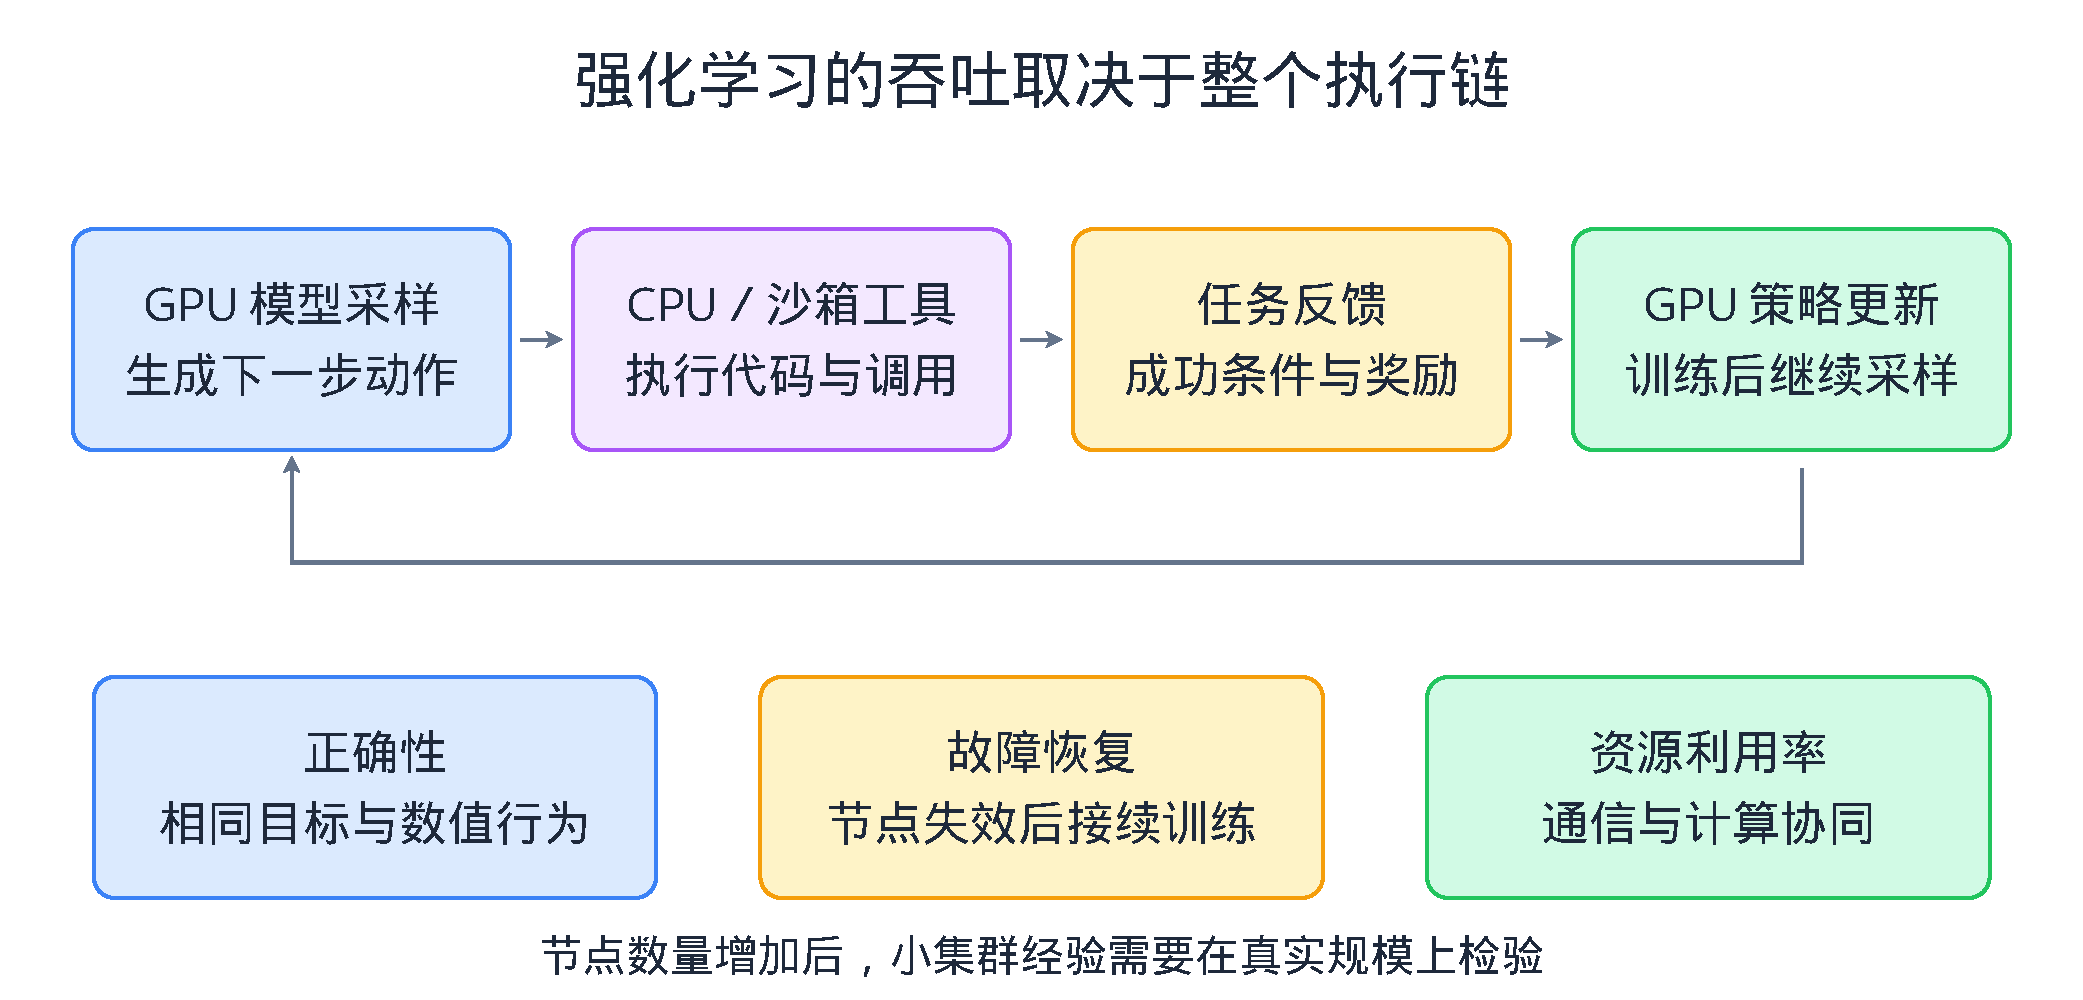
\includegraphics[width=\linewidth,height=.68\textheight,keepaspectratio]{assets/rl-system.pdf}
\caption{强化学习的吞吐取决于整个执行链；依据节目口述整理（00:25:05–00:27:23；00:42:03–00:45:29）}
\end{figure}
\begin{knowledgebox}{读图：从可执行环境到千卡训练系统}
图上半部分是由四个方框构成的闭环链路：从左到右依次为“GPU 模型采样（生成下一步动作）”指向“CPU／沙箱工具（执行代码与调用）”，再指向“任务反馈（成功条件与奖励）”，随后指向“GPU 策略更新（训练后继续采样）”，并由底部长箭头回流至最左侧的“GPU 模型采样”。图下半部分并列三个方框，列出集群扩展后的系统要求：“正确性（相同目标与数值行为）”、“故障恢复（节点失效后接续训练）”和“资源利用率（通信与计算协同）”，最下方文字提示“节点数量增加后，小集群经验需要在真实规模上检验”。
\end{knowledgebox}
该图直观说明了 CPU 沙箱并发与 GPU 计算共同制约着强化学习的整体吞吐，而在跨越算力规模时必须重新检验正确性、容错与利用率。下一章将转向研究者如何识别这些核心系统问题。
\needspace{6\baselineskip}\subsection{本章小结}
\begin{enumerate}
\item 智能体强化学习的吞吐受整条执行链制约：函数调用和代码执行依赖 CPU 与多容器沙箱的并发调度与低时延响应，同时需要合理的奖励设计与多轮用户模拟。
\item 组织内的数据汇集有助于后训练：英伟达内部的 NeMo Gym 通过收集各团队的智能体数据与强化学习环境，为 Nemotron 模型的强化学习训练提供了支持。
\item 算力规模跨越千卡、万卡后，系统必须应对容错恢复、精度匹配与维持 MFU 等挑战；Miles 框架结合商业合作完成了千卡级口述验证，并继续向万卡级优化推进。
\end{enumerate}
\needspace{8\baselineskip}\section{研究判断来自怎样的学习和转向}
前一章展示了强化学习从环境沙箱到千卡集群的工程全貌。一个值得深思的问题是：一位博士前四年深耕统计与机器学习理论的研究者，为何能在大模型浪潮初起时迅速转向底层基础设施？本章结合朱邦华在清华与伯克利的求学经历，剖析跨学科探索、学术评价体系与算力资源如何共同塑造研究者的技术判断力。
\needspace{6\baselineskip}\subsection{从通信和计算生物学走到统计}
研究者的方向选择往往伴随着对“什么问题能产生实际影响”的思考。朱邦华本科就读于清华大学电子工程系，最初接触通信领域的课题。大三暑假，他通过斯坦福大学与国内高校合办的本科生暑期科研项目 UGVR，前往斯坦福跟随通信领域学者 David Tse 开展研究。当时，David Tse 的研究兴趣正从通信转向计算生物学（Computational Biology，利用算法与统计模型处理基因测序拼接、基因组分析等生命科学问题的交叉学科）。

这次暑期科研促成了朱邦华的第一次研究转向。他觉得将深度学习等方法用于基因组预测（Genome Prediction）与基因拼接（Genome Assembly），有可能在基因与医疗探索上产生更直接的影响，因此申请博士时选择了计算生物学方向，并借此进入加州大学伯克利分校（UC Berkeley）。在回顾求学经历时，他用大语言模型的长上下文（Long Context）作自嘲，说自己属于考前突击看书就能考出好成绩、考完却容易忘光的类型，仿佛只把内容放进了临时上下文而没有变成脑子里的“权重”，隔段时间再看又能重新捡起来。

进入伯克利后，他的研究轨迹再次因学术合作网而转向。当时同为清华电子系校友的焦剑涛刚刚入职伯克利担任助理教授，研究重心在统计学（Statistics）与信息论（Information Theory）。朱邦华与焦剑涛以及同期入职的助理教授 Jacob Steinhardt 展开合作，并在统计机器学习泰斗 Michael I. Jordan（迈克尔·乔丹）的指导下，逐步深入统计理论、鲁棒统计与强化学习理论。从电子通信、计算生物学再到统计理论与博弈论，这几次看似跨度极大的迁移，让他得以观察不同学科如何定义核心问题，也为日后评估大模型技术方向积累了多维度的参照系。

\needspace{6\baselineskip}\subsection{ChatGPT 如何改变问题的重要性}
在博士圈子里，有时存在所谓“做理论的看不起做算法的，做算法的看不起做系统的”说法。在 00:47:24–00:49:42 的访谈中，朱邦华解释了自己为何在博士第五年从理论研究转向大语言模型与人工智能基础设施（AI Infra）：在他看来，随着大模型规模扩大，决定实际影响力的关键问题发生了变化。

他回顾道，在自己刚进入伯克利的阶段，所接触的机器学习问题规模相对较小，即便是当时工业界重要的大规模推荐系统（Recommendation System，根据用户历史行为预测偏好的信息过滤系统），其单模型规模与今天的大语言模型相比也有很大差异。在当时的研究环境下，算法设计与统计理论能够为许多机器学习问题提供直接指导，因此像 Michael I. Jordan 或 Martin J. Wainwright 这样研究统计与机器学习理论的学者，是许多学生向往的导师。

而在 ChatGPT 与大语言模型出现后，朱邦华感受到研究重心发生了转移。在高质量训练与合适配置下，扩大数据规模（Scale Data）、模型参数量（Scale Model Size）并升级底层基础设施，成为推动模型能力提升的重要趋势。此时，试图用纯理论去预测“模型能变得多聪明”对实际研发的帮助有限；相反，紧迫的问题变成了“如何以更低的成本把超大模型训练出来”。他举了一个假设性的算例来说明这种供需变化：如果训练一个超大模型原本需要花费 100 亿美元，而通过更好的基础设施能把成本降到 50 亿美元，这种系统工作对现实世界产生的直接影响就会非常可观。正是出于对现实影响力的看重，他决定转向后训练与底层系统研发。

\needspace{6\baselineskip}\subsection{代表作、研究文化与导师的判断逻辑}
在 00:55:22–01:01:51 谈及求学体验时，朱邦华对比了自己本科与伯克利博士阶段的个人感受：他觉得自己在国内读书时，常见的评价方式相对偏重平均学分绩点（GPA）、奖学金或社会工作等少数维度；而在伯克利读博期间，他感受到身边的同学与老师各自有不同的专长，学术评价更看重代表作的“最大值（Maximum）”，即一个人在博士期间哪怕只有一篇代表性论文，只要这项工作产生了广泛影响、被大家普遍使用，就会受到高度认可，而不必单纯追求每年发表论文的数量。

在这种研究氛围中，他对自己早期的判断也有过反思。朱邦华回忆，自己博一时曾与导师 Jacob Steinhardt 合写过一篇近两百页的鲁棒统计（Robust Statistics，研究数据存在异常或污染时如何保持可靠估计的统计学分支）论文并投往统计期刊《Annals of Statistics》。到了第二年，Steinhardt 转向“机器学习科学（Science of Machine Learning）”，研究模型可解释性与语言模型评测，并参与推出了 MMLU（Massive Multitask Language Understanding，大规模多任务语言理解基准，通过多学科问题测试语言模型知识与理解能力的评测集）。当时专注于理论证明的朱邦华一度无法理解为什么要拿常识问题去考语言模型；直到后来 MMLU 成为广泛使用的大模型评测基准，他才在事后体会到 Steinhardt 当初选择方向的前瞻性。

另一位导师 Michael I. Jordan 则向他展示了顶尖学者如何保持知识更新与推导未来。尽管早已享誉学界且年事渐高，Jordan 依然坚持每周参加两个半小时的读书会（Reading Group），带着学生逐字研读他自己尚不熟悉的新领域专著。因为判断未来属于人机交互与协作，而理解人类行为与激励机制本质上是经济学问题，Jordan 便带领课题组连续数年研读优化理论、博弈论（Game Theory）与拍卖理论（Auction Theory）。从心理学博士起步，自学统计、开拓机器学习，再到结合经济学，Jordan 从不把自己局限在既有的学术标签内。朱邦华由此总结道，跟随这些大师最大的收获，是观察他们如何摆脱短期热点的跟风，依靠一套自洽的底层逻辑去推导未来五到十年真正重要的问题。

\needspace{6\baselineskip}\subsection{探索与资源怎样塑造能力}
如果把视野拉长到整个青年阶段的研究与创业，过往那些看似“放弃”了的学科探索究竟留下了什么？在 01:25:00–01:28:52 的回顾中，朱邦华表示，如果回到 25 岁，他依然会选择多去尝试不同的新方向。正是因为亲身涉足过通信、计算生物学、区块链理论、经济学博弈论以及统计机器学习，亲眼见过不同研究方向的兴起与式微，他才能建立起更完备的认知图谱——清楚地知道每个学科到底在解决什么核心矛盾，为什么某些问题在过去至关重要而今天退居次席，又为什么另一些曾被忽视的问题在今天成了时代的核心。

这种对方向的判断力同样会在合作与产品实践中得到修正。朱邦华在访谈中对照了自己与 RadixArk 联合创始人盛颖在几次决策上的不同判断：盛颖在参与发起 Chatbot Arena 时，就判断模型盲测对比会成为广泛需求；后来在开源推理引擎 vLLM 已经做得很好的情况下，朱邦华起初认为没有必要再做 SGLang，而盛颖则认为只要从第一性原理出发把推理速度、稳定性和支持范围做好，并尽早布局与强化学习的结合，用户就会选择它。最终社区的发展印证了盛颖的判断。能够根据实验观察与社区反馈承认并修正自身看法的局限，也是研究与工程判断走向成熟的一部分。

面对正在读博或思考去向的年轻学生，朱邦华结合自身经历谈了两点看法（01:02:18–01:06:52）：
\begin{itemize}
\item 刚读博的同学不必因前两三年没有突出成果而过度焦虑：他本人是在博士第五年才转向大模型方向，导师 Jacob Steinhardt 也是在博士第五年才做出后来求职伯克利教职的代表性鲁棒统计论文。
\item 在学术界与工业界之间做选择时，需要考虑研究问题对资源的依赖：朱邦华本人在博士毕业季申请并拿到了华盛顿大学（University of Washington）的教职，截至访谈时处于推迟入职（Defer）状态。他指出，在大模型与智能体方向上，许多探索依赖算力与词元（Token）消耗——例如他举例说，在公司里研究员每月使用两万美元额度的 Claude Code 去探索智能体协作是可能的，而在高校里这样的开销很容易耗尽年轻教师的经费。因此，如果有机会进入算力与工具资源更充足的环境接触前沿问题，对培养这一方向的实践直觉会有很大帮助。
\end{itemize}

\begin{importantbox}{为什么大模型规模扩展提升了系统工程的权重}
朱邦华从理论转向 AI 基础设施（AI Infra），源于研究问题约束条件的变化。在他早期接触的机器学习课题中，单模型规模相对较小，统计理论与算法设计能够直接指导训练。而在大语言模型时代，随着参数量与数据量大幅扩展，如何降低超大规模训练与推理的成本成为关键瓶颈。正如他用“将假设的百亿美元训练成本降至五十亿美元”所比喻的，底层系统效率的改善能够在大规模算力投入中产生直接的现实影响。
\end{importantbox}
\begin{warningbox}{用实证观察修正学科偏见}
在科研与技术演进中，研究者容易受限于既有的评价习惯或学科视角：
\begin{enumerate}
\item 重代表作影响而非单纯比拼数量：在学术研究中，一项真正解决关键问题或被广泛采用的工作（Maximum），往往比单纯累加常规论文数量更能体现研究价值。
\item 避免用旧范式过早否定新探索：例如在语言模型早期，MMLU 等评测工作曾被偏重纯理论的研究者低估，SGLang 初期也曾被认为难以在已有引擎之外打开局面。面对新方向时，结合实验结果与真实使用反馈及时修正判断，有助于跳出原有背景的局限。
\end{enumerate}
\end{warningbox}
\begin{table}[H]\centering\small
\caption{朱邦华学术经历中的关键研究方向转向与判断逻辑对比}
\begin{tabular}{>{\raggedright\arraybackslash}p{\dimexpr(\linewidth-6\tabcolsep)/3\relax}>{\raggedright\arraybackslash}p{\dimexpr(\linewidth-6\tabcolsep)/3\relax}>{\raggedright\arraybackslash}p{\dimexpr(\linewidth-6\tabcolsep)/3\relax}}
\toprule
阶段与领域 & 核心关注的问题 & 转向契机与对研究判断的塑造\\\midrule
通信与计算生物学 (清华 / 斯坦福 UGVR) & 信号传输理论；利用深度学习进行基因预测与序列拼接 & 跟随 David Tse 暑期科研，体会到将计算工具用于生命科学能产生直接的现实影响\\[4pt]
统计、信息论与鲁棒统计 (伯克利博士前期) & 数据污染下的可靠统计估计、强化学习与博弈论数学理论 & 与焦剑涛、Jacob Steinhardt 及 Michael I. Jordan 合作，习得顶尖学者推导长远问题的逻辑与跨界读书习惯\\[4pt]
MMLU 与早期语言模型评测 (导师 Steinhardt 的转向) & 通过大规模多任务学科测试评估语言模型的知识与理解能力 & 起初因偏重理论而低估其意义，后见证 MMLU 成为广泛使用的评测基准，体会到前瞻性实证工作的价值\\[4pt]
大模型后训练与 AI Infra (博士第五年至今) & 以高可靠性与低成本完成大规模 RLHF/RLVR 训练及高吞吐推理 & 试用 ChatGPT 后意识到算法与系统尚有巨大优化空间，判断算力与系统效率已成为释放智能潜力的核心杠杆\\[4pt]
\bottomrule\end{tabular}\end{table}
回顾朱邦华从通信、计算生物学、统计理论到大模型基础设施的多次转向，以及他与合作者在开源项目上的决策对照，可以看到研究者的技术判断力并非一蹴而就，而是在持续探索与外部反馈中逐步校准的。
\begin{figure}[H]\centering
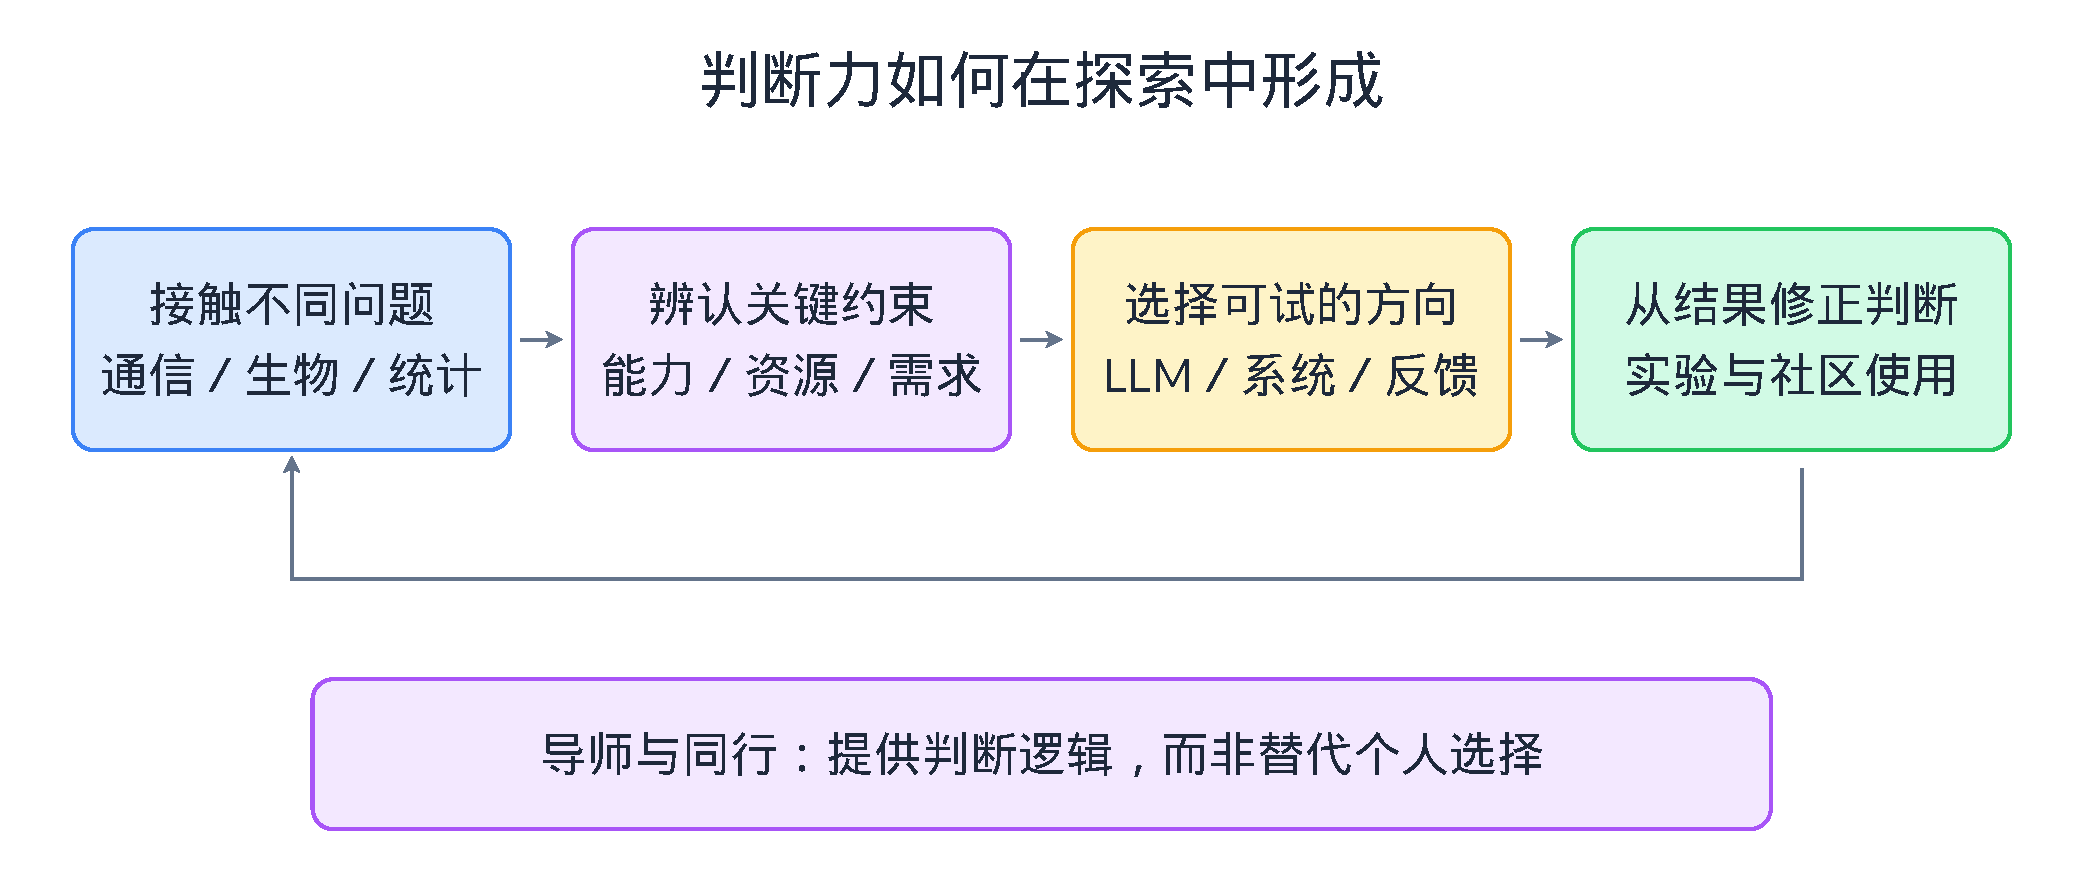
\includegraphics[width=\linewidth,height=.68\textheight,keepaspectratio]{assets/research-decision.pdf}
\caption{判断力如何在探索中形成；依据节目口述整理（00:49:53–01:07:02；01:25:00–01:28:52）}
\end{figure}
\begin{knowledgebox}{读图：研究判断来自怎样的学习和转向}
图上方四个方框从左到右通过箭头依次连接：“接触不同问题（通信／生物／统计）”指向“辨认关键约束（能力／资源／需求）”，再指向“选择可试的方向（LLM／系统／反馈）”，最后指向“从结果修正判断（实验与社区使用）”。一条回流箭头从最右侧方框底部引出并指回最左侧的“接触不同问题”，构成持续迭代的循环。图下方设有一个独立横框，注明：“导师与同行：提供判断逻辑，而非替代个人选择”。
\end{knowledgebox}
这一循环结构表明，跨学科视野与导师同行的思考方式提供了分析约束的框架，但最终仍需通过真实实验与社区使用结果来修正个人判断。下一章将具体考察他对训练范式与多模态演进的技术判断。
\needspace{6\baselineskip}\subsection{本章小结}
\begin{enumerate}
\item 跨学科探索有助于理解不同问题的约束：从通信、计算生物学到统计理论与博弈论，多领域的尝试帮助研究者看清不同研究方向的兴衰逻辑。
\item 研究判断体现在代表作追求与长远推导上：无论是 Jacob Steinhardt 参与布局 MMLU 评测，还是 Michael I. Jordan 持续研读经济学以思考人机协作，都展示了推导长远问题的思考方式。
\item 大模型时代使系统成本与资源条件成为重要约束：研究者应结合自身感兴趣的问题与算力、工具资源做出路径选择，并在实验与社区反馈中不断校准判断。
\end{enumerate}
\needspace{8\baselineskip}\section{预训练、持续学习与多模态的下一步}
前一章梳理了研究者的学术训练如何转化为对大模型趋势的判断力。当目光投向未来一到五年的技术演进时，预训练与后训练的职责边界正在重塑，持续学习的探索悄然兴起，而纯文本模型也逐步向原生多模态、世界模型与机器人方向延伸。本章结合访谈中的技术展望，解析各训练阶段的协同机制与下一代模型对底层基础设施提出的新课题。
\needspace{6\baselineskip}\subsection{预训练提供怎样的基础}
在大语言模型的训练流程中，预训练与后训练各自承担着不同的角色。在 01:09:28–01:11:08 的讨论中，朱邦华指出，不同前沿实验室对各阶段潜力的看法不完全相同，而在他看来，预训练阶段的数据清洗质量依然非常重要。

为什么预训练的数据工作还没有遇到明显瓶颈？因为预训练为模型打下了底层表征与知识基础。朱邦华举例说，如果能把预训练数据清洗得更好，或者加入更多高质量的编程数据（Coding Data），模型的能力边界还能继续提升。按照他的研究直觉，预训练在很大程度上影响了后训练能够达到的上限空间。

当然，把预训练看作“决定后训练边界”是研发中的经验概括，并非严格数学意义上的固定上界。在实际训练中，预训练与后训练相互配合：做好预训练语料的清洗与高质量数据补充，能够为后续的微调与强化学习提供更好的起点。

\needspace{6\baselineskip}\subsection{SFT、RL 和 on-policy distillation}
在预训练之后，后训练阶段包含监督微调（SFT）、强化学习（RL）以及蒸馏等环节。在朱邦华看来，现在的 SFT 更像是对预训练模型做一层小幅修正：利用质量更高的数据，让模型具备基本的指令遵循（Instruction Following）能力与回答规范，减轻预训练语料中低质量数据带来的影响。

在此之后，开展强化学习（RL）训练的目标，是把模型能力尽可能推向预训练所奠定的潜力边界。而在不同领域分别训练出表现较好的专家模型（Expert Model）后，如果希望将它们合并回一个综合表现均衡的通用模型（Generalist Model），朱邦华提到了当前常被讨论的同策略蒸馏（On-policy Distillation）。

同策略蒸馏不同于把多个模型的参数权重直接做算术平均，也不同于只用静态教师语料做离线微调。它的基本机制是由学生模型（Student Model）在当前策略下自己采样生成轨迹（即保持 On-policy），再由一个或多个教师模型（Teacher Model）针对这些轨迹提供概率分布或指导信号，以此减轻训练与实际生成时的分布偏移，并将多个专项专家模型的能力整合到一个通用模型中。

\needspace{6\baselineskip}\subsection{持续学习与研发反馈回路}
谈到最近一两年的前沿问题（01:07:02–01:08:40），朱邦华指出，许多新成立的实验室（Neo Labs）都在探索持续学习（Continual Learning，又称 Continuous Learning，一般指模型在持续到来的新数据或新任务上不断学习新能力、同时保持已有能力的学习范式，既包括在线更新也包括分阶段更新）。他坦言，目前业界对什么场景和范式算作持续学习，定义还不完全清晰。

例如，有人认为 Anthropic 在某种意义上展现了持续学习的效果：工程师们使用最新的 Claude Code 智能体去改进底层训练基础设施、提升数据质量，再用来训练下一代更强的模型。从机制上看，需要把这种“用当前模型辅助研发、改善系统与数据以训练下一代模型”的研发反馈回路（R\&D Feedback Loop），与直接改变当前模型权重或仅更新输入上下文的做法区分开来。朱邦华提出，如果这种研发正反馈在某个时刻迎来拐点并呈指数级加速，最先到达拐点的公司就可能实现较大幅度的能力跃升。

对于这种自我迭代能否一路通向人工超级智能（Artificial Superintelligence, ASI，假想中在广泛智力任务上远超人类水平的智能形态），朱邦华保持了审慎态度。他表示，即便这一机制能够跑通，在现实中仍可能受制于计算资源与能源供给（Energy Constraints），未必能无限制地爆发。此外，在 01:20:02–01:21:07 谈及各类新兴实验室时，他也提到像强化学习学者 David Silver 的团队正尝试跳出“预训练加后训练”的现有范式，探索从零开始做强化学习（RL from scratch）的思路。虽然还不确定这类尝试最终能否成功，但更多团队探索新范式有助于推动技术边界。

\needspace{6\baselineskip}\subsection{多模态、世界模型与机器人}
如果把眼光放到五年之后，朱邦华个人认为，纯文本语言模型（Pure Text Language Model）的相对重要性可能会下降，更多探索会走向原生多模态（Native Multimodality）乃至全模态模型（Omni Model，能够接收任意模态输入并生成任意模态输出的模型），同时机器人学（Robotics）也会有新的进展。多模态会带来不同于纯文本的数据形态、交互方式与训练范式。例如在 01:23:25–01:24:14 谈到的世界模型（World Model）方向上，尽管具体定义尚有不同看法，但其重要目标是更好地预测物理世界的变化（Predict Physical World）或生成高质量的物理仿真环境（Physical Simulation Environments），这对机器人训练乃至游戏开发都很有帮助。

当模型应用延伸到机器人领域时，像 SGLang 这样的推理引擎能否发挥作用？在 01:14:12–01:15:11 的交流中，朱邦华表示这取决于机器人的具体使用场景。如果机器人运行的是对话模型或视觉-语言-动作模型（Vision-Language-Action, VLA，结合视觉与语言输入并输出动作控制的模型），在某些预填充负担较重（Prefill-heavy，即在生成输出前并行处理输入特征与上下文的计算占比较高）的设置下，推理系统需要针对具体硬件、模型架构与输入负载做专门优化。

不过他也指出，推理引擎底层的许多核心逻辑——例如算子内核（Kernel，在 GPU 等硬件上执行的底层计算子程序）与编译器（Compiler，将计算图转化为底层可执行代码的工具）——依然可以跨场景复用。至于基础设施更长远的演进，朱邦华表示目前机器人的合作还处于早期，而团队希望在支持多模态与智能体演进的过程中，逐步探索开放平台与前沿基础设施结合的可能性。

\begin{knowledgebox}{同策略蒸馏（On-policy Distillation）是如何工作的}
当团队希望将多个领域专家模型（Expert）的能力整合进一个通用模型（Generalist），或用教师模型指导学生模型时，同策略蒸馏采用以下机制：
\begin{enumerate}
\item 学生同策略采样：由学生模型在自身当前策略下生成回答序列，使训练样本分布与学生模型实际推理时的分布保持一致，减轻分布偏移。
\item 教师信号指导：由一个或多个领域专家教师模型在学生生成的这些轨迹上提供概率分布或评估指导，避免直接对不同模型的参数权重做简单平均，从而将多领域特长整合到同一个学生模型中。
\end{enumerate}
\end{knowledgebox}
\begin{warningbox}{区分学习发生的三个层次}
在讨论模型能力演进与“持续学习”时，可以按改变的对象区分三个不同层次：
\begin{enumerate}
\item 更新模型权重：通过预训练、SFT、RL 或蒸馏直接改变神经网络参数，包括在持续到来的新数据上分阶段或在线更新权重。
\item 改变输入上下文：模型权重保持不变，仅在推理时通过长上下文或外部检索注入新信息。
\item 研发反馈回路（R\&D Feedback Loop）：研究人员使用当前模型（如 Claude Code）辅助改代码、优化基础设施与清洗数据，再去训练下一代模型；这一循环加速了跨版本的研发迭代，但受计算资源与能源条件制约。
\end{enumerate}
\end{warningbox}
\begin{table}[H]\centering\small
\caption{大模型训练各阶段与未来演进方向的技术机制对比}
\begin{tabular}{>{\raggedright\arraybackslash}p{\dimexpr(\linewidth-6\tabcolsep)/3\relax}>{\raggedright\arraybackslash}p{\dimexpr(\linewidth-6\tabcolsep)/3\relax}>{\raggedright\arraybackslash}p{\dimexpr(\linewidth-6\tabcolsep)/3\relax}}
\toprule
技术阶段或演进方向 & 解决的核心问题 & 工作机制与系统实践关系\\\midrule
预训练 (Pre-training) & 构建模型的基础知识储备与底层表征能力 & 依赖大规模高质量数据清洗（如优质代码语料），其质量直接影响后续训练可挖掘的潜力空间\\[4pt]
监督微调 (SFT) 与强化学习 (RL) & 学习指令遵循与任务示范，并通过反馈激发推理与工具调用能力 & SFT 用高质量示范数据做微调修正；RL 在环境或奖励引导下挖掘预训练底座的潜力\\[4pt]
同策略蒸馏 (On-policy Distillation) & 将多个垂直领域专家模型的能力融合进单一通用模型 & 在学生模型自身采样生成的轨迹上引入教师指导信号，减轻分布偏移，整合多领域专家能力\\[4pt]
全模态 (Omni)、世界模型与 VLA & 突破纯文本局限，实现跨模态实时交互、物理世界模拟与机器人控制 & 部分场景存在预填充较重（Prefill-heavy）等负载特点并需适配新硬件，但底层算子（Kernel）与编译器（Compiler）可复用\\[4pt]
\bottomrule\end{tabular}\end{table}
在讨论预训练、后训练与当前热门的“持续学习”时，容易将模型权重的直接训练流程与“用强模型辅助工程师改进代码和数据”的研发循环混为一谈。下图将这两个不同层次的机制放在同一视图中进行对比。
\begin{figure}[H]\centering
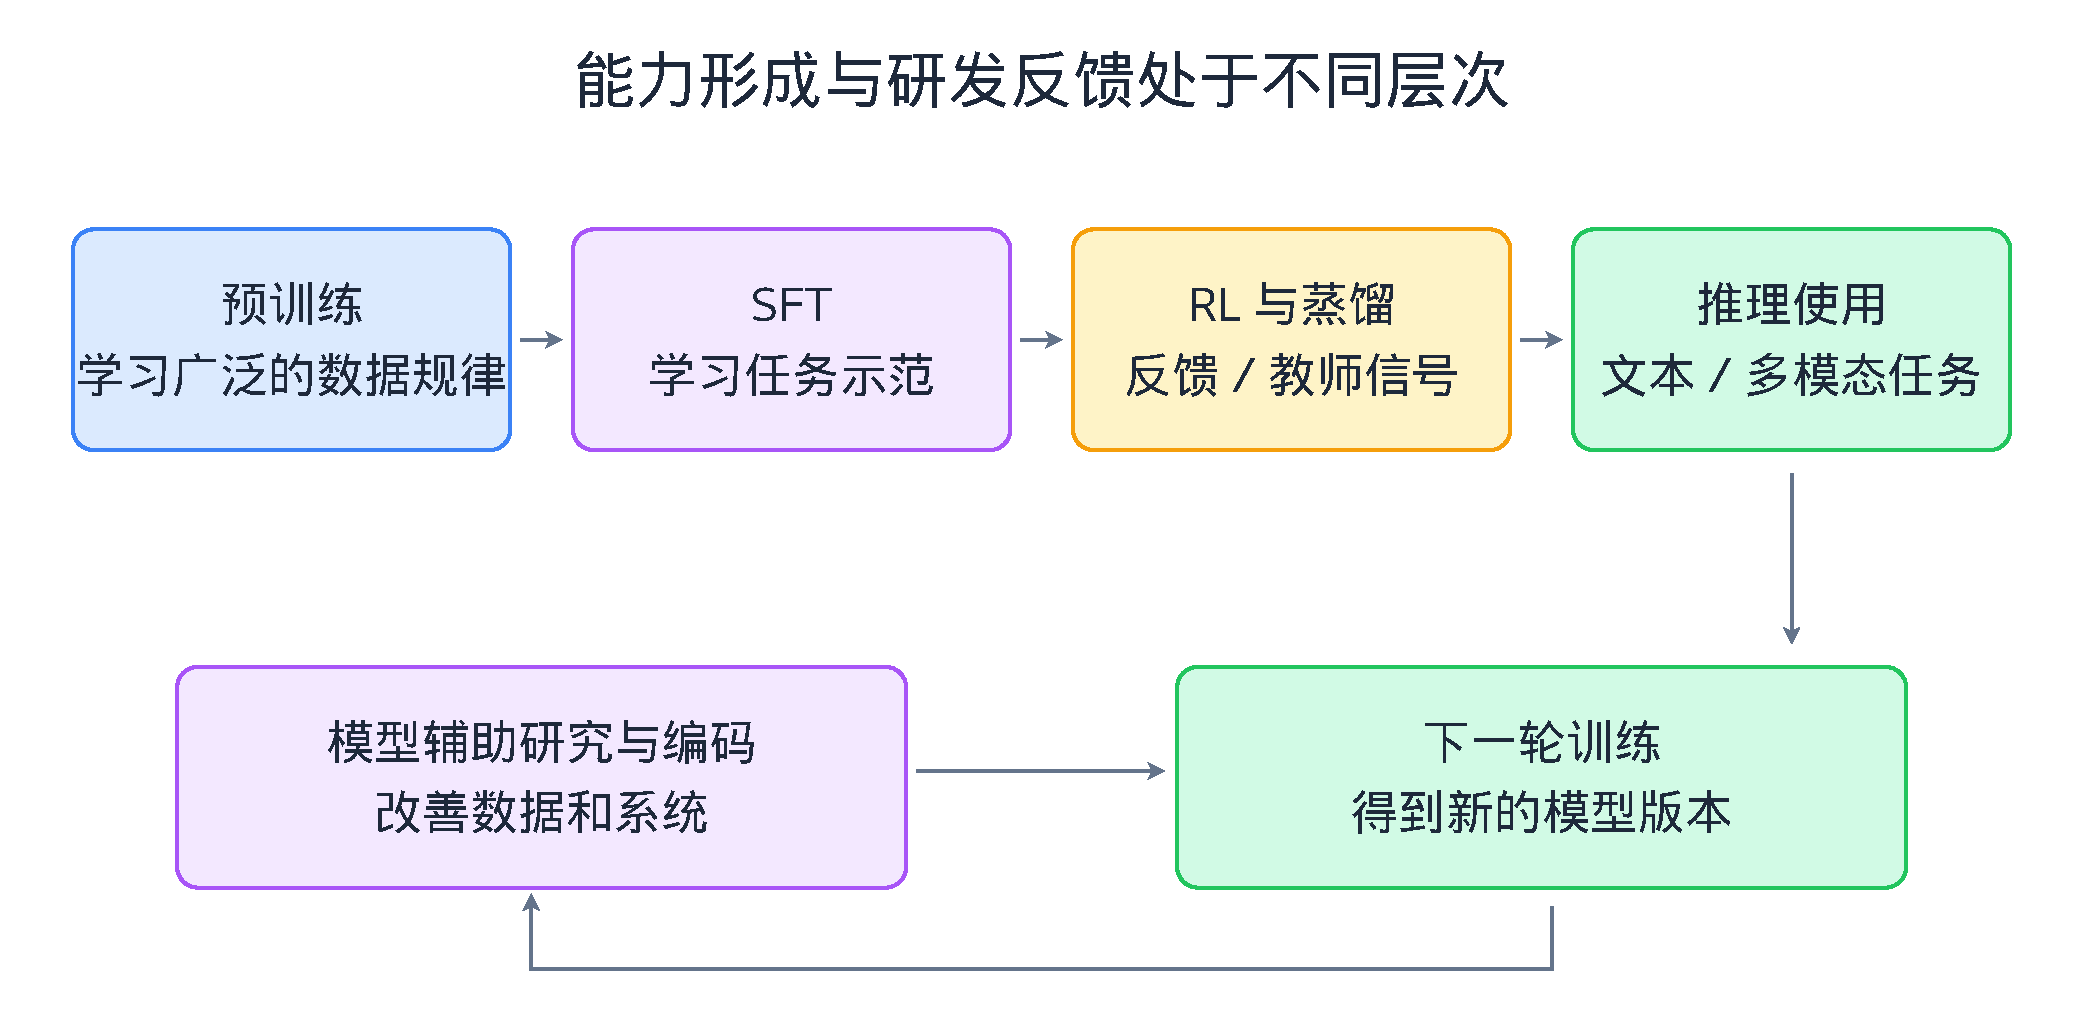
\includegraphics[width=\linewidth,height=.68\textheight,keepaspectratio]{assets/learning-layers.pdf}
\caption{能力形成与研发反馈处于不同层次；依据节目口述整理（01:07:17–01:11:08）}
\end{figure}
\begin{knowledgebox}{读图：预训练、持续学习与多模态的下一步}
图形分为上下两层。上层四个方框从左到右由箭头连接，表示模型能力形成的训练与使用流程：“预训练（学习广泛的数据规律）”指向“SFT（学习任务示范）”，再指向“RL 与蒸馏（反馈／教师信号）”，最后到达“推理使用（文本／多模态任务）”。从最右侧“推理使用”底部有一条向下箭头指向下层区域。下层由两个宽框构成闭环：左侧“模型辅助研究与编码（改善数据和系统）”指向右侧“下一轮训练（得到新的模型版本）”，底部回流箭头再从“下一轮训练”指回左侧方框。
\end{knowledgebox}
上下两层的区分清楚表明，模型在推理使用中辅助研发人员改善数据与系统、进而推动下一轮训练，属于研发流程层面的正反馈循环，不同于在单次部署中直接改变模型权重的训练过程。
\needspace{6\baselineskip}\subsection{本章小结}
\begin{enumerate}
\item 预训练与后训练相互配合：预训练的数据清洗质量影响模型的潜力空间；SFT 负责规范基本的指令遵循，RL 负责挖掘能力上限，同策略蒸馏则通过在学生自身生成轨迹上引入教师指导来整合多个专家模型。
\item 理解持续学习需明确作用层次：用现有模型辅助优化基础设施与数据构成了跨版本的研发反馈回路，但仍受算力与能源制约；同时新兴实验室也在探索从零开始强化学习等不同范式。
\item 面向未来五年，朱邦华判断多模态、世界模型与机器人方向将带来更多新问题；虽然部分 VLA 等场景需要对预填充负载与硬件做专门适配，但推理引擎底层的算子与编译技术仍可复用。
\end{enumerate}
\needspace{8\baselineskip}\section{开源社区怎样连接研究与创业}
前一章探讨了预训练、持续学习与多模态的技术演进方向。然而，前沿研究要真正转化为广泛使用的生产力，离不开技术商业化与开源生态的协同。本章结合朱邦华从 Nexusflow 到英伟达再到创立 RadixArk 的历程，解析技术方向与市场时机的关系、开源社区如何与商业服务相互赋能，以及基础设施公司从解决具体痛点走向开放平台的路径。
\needspace{6\baselineskip}\subsection{技术方向对了，市场也需要时机}
在人工智能创业中，除了判断技术趋势，还需要踩准市场接受的时间节点（Timing）。在 00:39:45–00:41:09 回顾第一次创业 Nexusflow AI 的经历时，朱邦华谈到了一条切身体会：在合适的时间做正确的事至关重要。2023 年团队切入企业级智能体（Enterprise Agents）与函数调用（Function Calling）方向时，虽然看准了技术演进趋势，但当时的企业市场尚未完全准备好。

为什么技术判断超前反而会带来商业阻力？原因在于当时的客户普遍混淆了检索增强生成（Retrieval-Augmented Generation, RAG，在生成回答前先从外部知识库检索相关文档片段、将其作为上下文输入模型以提升回答准确性的技术）与智能体（Agent）的概念。当团队向客户介绍智能体时，许多企业误以为那只是搜索一下文本再生成回答的 RAG 系统。为了消除这种认知偏差，初创团队不得不耗费大量精力去教育市场，向客户解释智能体不仅能检索信息，还能采取行动（Take Action）、调用外部工具（Tool Use），并在多轮交互（Multi-turn Interaction）中持续把工具用好。

从机制上看，RAG 与智能体解决的是不同层面的问题：RAG 是检索增强的技术机制，核心在于从外部知识库或接口获取信息并放入上下文，供模型生成有据可依的回答（检索来源既可以是静态文档，也可以是动态信息，并不局限于特定数据库形式）；而智能体的核心在于围绕任务目标自主决定下一步行动，通过多轮调用外部工具或执行操作来完成任务（这些行动既可能是查询获取信息，也可能是修改外部系统状态），在实际系统中二者经常结合使用。由于 2023 年市场对多轮工具调用的需求尚未全面爆发，早期入场的团队不得不花大量时间做市场教育，反而是稍晚进入市场的团队更容易赶上需求成熟期。

\needspace{6\baselineskip}\subsection{从第一次收购到第二次创业}
随着 DeepSeek 相关进展让业界更加重视可验证奖励强化学习（RLVR），Nexusflow AI 在后训练与工具调用上的积累迎来了转折，于 2025 年被英伟达收购。正如第 3 章所述，这次并购让团队从只有 2 到 4 个节点（按 8 卡节点计为 16 到 32 张 H100 GPU）的初创状态，进入了算力充裕的大厂环境，并推动了 NeMo Gym 等内部项目。

在英伟达工作数月后，朱邦华于 2025 年 12 月选择离开，与长期合作者盛颖共同创立 RadixArk。访谈中主持人提到这次离开意味着放弃了收购带来的不少未归属收益——关于具体数额，朱邦华表示不便透露，仅坦言原本已足够安稳生活。谈及再次创业的原因，他表示吸引自己的是开源社区的技术与人，以及新公司希望推进的使命，这一决定也得到了家人与前同事的理解和支持。

据主持人介绍，RadixArk 获得了 1 亿美元融资，估值超过 4 亿美元。需要注意，风险投资的融资额与估值反映的是资本市场对团队与未来潜力的投入预期，并不等同于公司已经实现的业务营收。在朱邦华看来，当前投资人与公司之所以愿意投入资金支持新兴实验室（Neo Labs）与算力基础设施，是因为大家都在押注通用人工智能方向的演进机会，这些资金能够转化为人才聚集与算力资源，推动更多前沿尝试。

\needspace{6\baselineskip}\subsection{社区普及与商业服务的相互支持}
在开启第二次创业时，如何处理开源社区与商业化之间的关系，是基础设施公司必须回答的核心问题。在 01:12:32–01:14:12 的讨论中，朱邦华剖析了纯开源社区在面对前沿强化学习训练时的天然局限：要训练万亿参数规模（Trillion-level）的模型，必须依赖成千上万张 GPU 的集群来验证系统的可靠性与精度边界；然而，单纯依靠松散的开源社区，根本无力承担千卡乃至万卡级别的测试成本。

这正是商业公司与开源生态能够形成互补闭环的地方。通过 RadixArk 的商业合作与资金支持，工程团队得以在真实的大规模集群上锤炼开源框架（例如强化学习框架 Miles 已经在千卡级别完成了可靠性验证，并继续向万卡规模的容错与调度优化推进），再将经过大规模检验的基础能力回馈给社区，从而实现前沿基础设施的普及化（Democratize，让原本只有顶尖巨头才能拥有的技术能力被更广泛的开发者和企业低成本获取）。

既然核心框架陆续开源，团队如何考虑哪些工作开源、哪些不开源？在 01:13:34–01:14:12 的回答中，朱邦华表示，团队希望尽可能降低大家在常见场景中使用前沿基础设施的成本与门槛；而对于某些极端场景下所需的极端优化（Extreme Optimization），有时开源出来对整个社区的帮助并不大。当主持人追问这是否也是保证商业模式的技巧时，朱邦华明确回应说，这不一定是保证商业模式的技巧，只是因为那些针对极端场景的优化就算开源，实际会用到的人也不多。节目中并未展开完整的收费或商业化细则，其核心取舍逻辑在于功能的通用使用面与社区实际价值。

\needspace{6\baselineskip}\subsection{成为平台之前先解决具体问题}
从解决当下具体工程痛点出发，RadixArk 沿着前文梳理的“推理到强化学习后训练”路径推进产品与合作。那么在更长远的未来（01:15:14–01:19:59），这类推理与强化学习基础设施会走向怎样的形态？朱邦华认为，在某个阶段，行业里可能会出现类似 Databricks 或 Snowflake 那样的平台型公司，赋能更多团队使用前沿级别的基础设施开展训练与推理。

而再往后看，他认为行业终局存在不同的可能性：一种可能是少数巨头公司既做模型又做基础设施，一骑绝尘，所有智能体都运行在单一公司的 API 之上；而他们更希望看到的另一种可能，是由不同公司构建的多样化智能体相互协作的生态。

在后一种愿景中，未来许多公司的运转与个人事务都可能通过智能体来完成——不仅有人类发布任务雇佣智能体，甚至在一些开源社区的早期探索中（如节目提及的 OpenClaw 衍生社区），还出现了智能体出资派人去线下办事的交互尝试。朱邦华设想，如果未来存在大量个人智能体（Personal Agents）与企业智能体，就需要定义智能体之间、以及智能体与人之间的交互接口（Interface），并由一家类似“电力公司”的底层平台去支撑它们的运行。为此，RadixArk 既希望成为开放的基础设施平台，也希望作为一家“基础设施优先（Infra-first）”的前沿实验室，去探索这些尚未定型的下一代交互与系统问题。

\begin{knowledgebox}{检索增强生成（RAG）与智能体（Agent）的机制差异}
在 2023 年的市场早期，不少企业容易将智能体与 RAG 混为一谈。二者可以结合使用，但机制重心不同：
\begin{enumerate}
\item 检索增强生成（RAG）：一种通过外部检索补充上下文的技术机制。系统先从文档库或接口中检索相关信息并拼接到输入中，帮助模型依据外部资料生成回答。
\item 智能体（Agent）：一种围绕目标自主决定行动步骤的执行方式。模型在多轮交互（Multi-turn）中输出函数调用（Function Calling）指令、使用外部工具或执行代码，并根据环境返回的反馈调整下一步动作。
\end{enumerate}
\end{knowledgebox}
\begin{warningbox}{理解开源测试条件与代码开放范围}
在分析 AI 基础设施的开源与商业互动时，需注意两个事实边界：
\begin{enumerate}
\item 融资估值与业务营收不同：节目提及的 1 亿美元融资与超过 4 亿美元估值属于风险投资的资金投入与估值预期，不等同于已实现的营业收入。
\item 开源范围取决于通用使用价值：松散的开源社区难以独立负担千卡、万卡级别的测试，商业项目能为开源框架（如 Miles）提供大规模验证条件；而针对极端场景的特定优化由于普通用户很少用到、对社区帮助有限，未必适合全部放入通用开源仓库，朱邦华也明确表示这并非单纯为了保留商业模式的技巧。
\end{enumerate}
\end{warningbox}
\begin{table}[H]\centering\small
\caption{AI 基础设施各业务层次与开源商业协同机制对比}
\begin{tabular}{>{\raggedright\arraybackslash}p{\dimexpr(\linewidth-6\tabcolsep)/3\relax}>{\raggedright\arraybackslash}p{\dimexpr(\linewidth-6\tabcolsep)/3\relax}>{\raggedright\arraybackslash}p{\dimexpr(\linewidth-6\tabcolsep)/3\relax}}
\toprule
系统层次或机制 & 解决的核心问题 & 机制特征与商业实践关系\\\midrule
推理基础设施 (如 SGLang) & 支撑模型高频在线服务，降低延迟与单次调用成本 & 市场需求最广、商业落地最直接；在服务过程中自然沉淀大量真实交互数据\\[4pt]
后训练与强化学习系统 (如 Miles) & 利用私有业务数据或环境反馈，定制化提升专项 Agent 能力 & 成本低于预训练而针对性强；与推理引擎配合形成“推理攒数据—训练提能力”的商业闭环\\[4pt]
开源社区与商业化的协同 & 弥合纯开源社区算力不足与前沿万亿模型大规模验证之间的鸿沟 & 借助商业项目支撑千卡/万卡级可靠性测试并将通用能力开源；仅面向极端场景、受众极少的优化则未必放入通用开源库\\[4pt]
Infra-first 平台与智能体网络愿景 & 避免单一巨头垂直垄断，支撑跨公司多元智能体的高频协作 & 先提供媲美前沿实验室的训练推理平台，长远探索个人/企业智能体交互接口与“电力公司”式底层赋能\\[4pt]
\bottomrule\end{tabular}\end{table}
前沿强化学习与推理基础设施需要大规模集群来验证可靠性，而单纯依靠松散的开源社区很难承担千卡、万卡的测试开销。RadixArk 试图通过开源社区与商业项目的互动来弥合这一差距，下图概括了二者的资源交换关系。
\begin{figure}[H]\centering
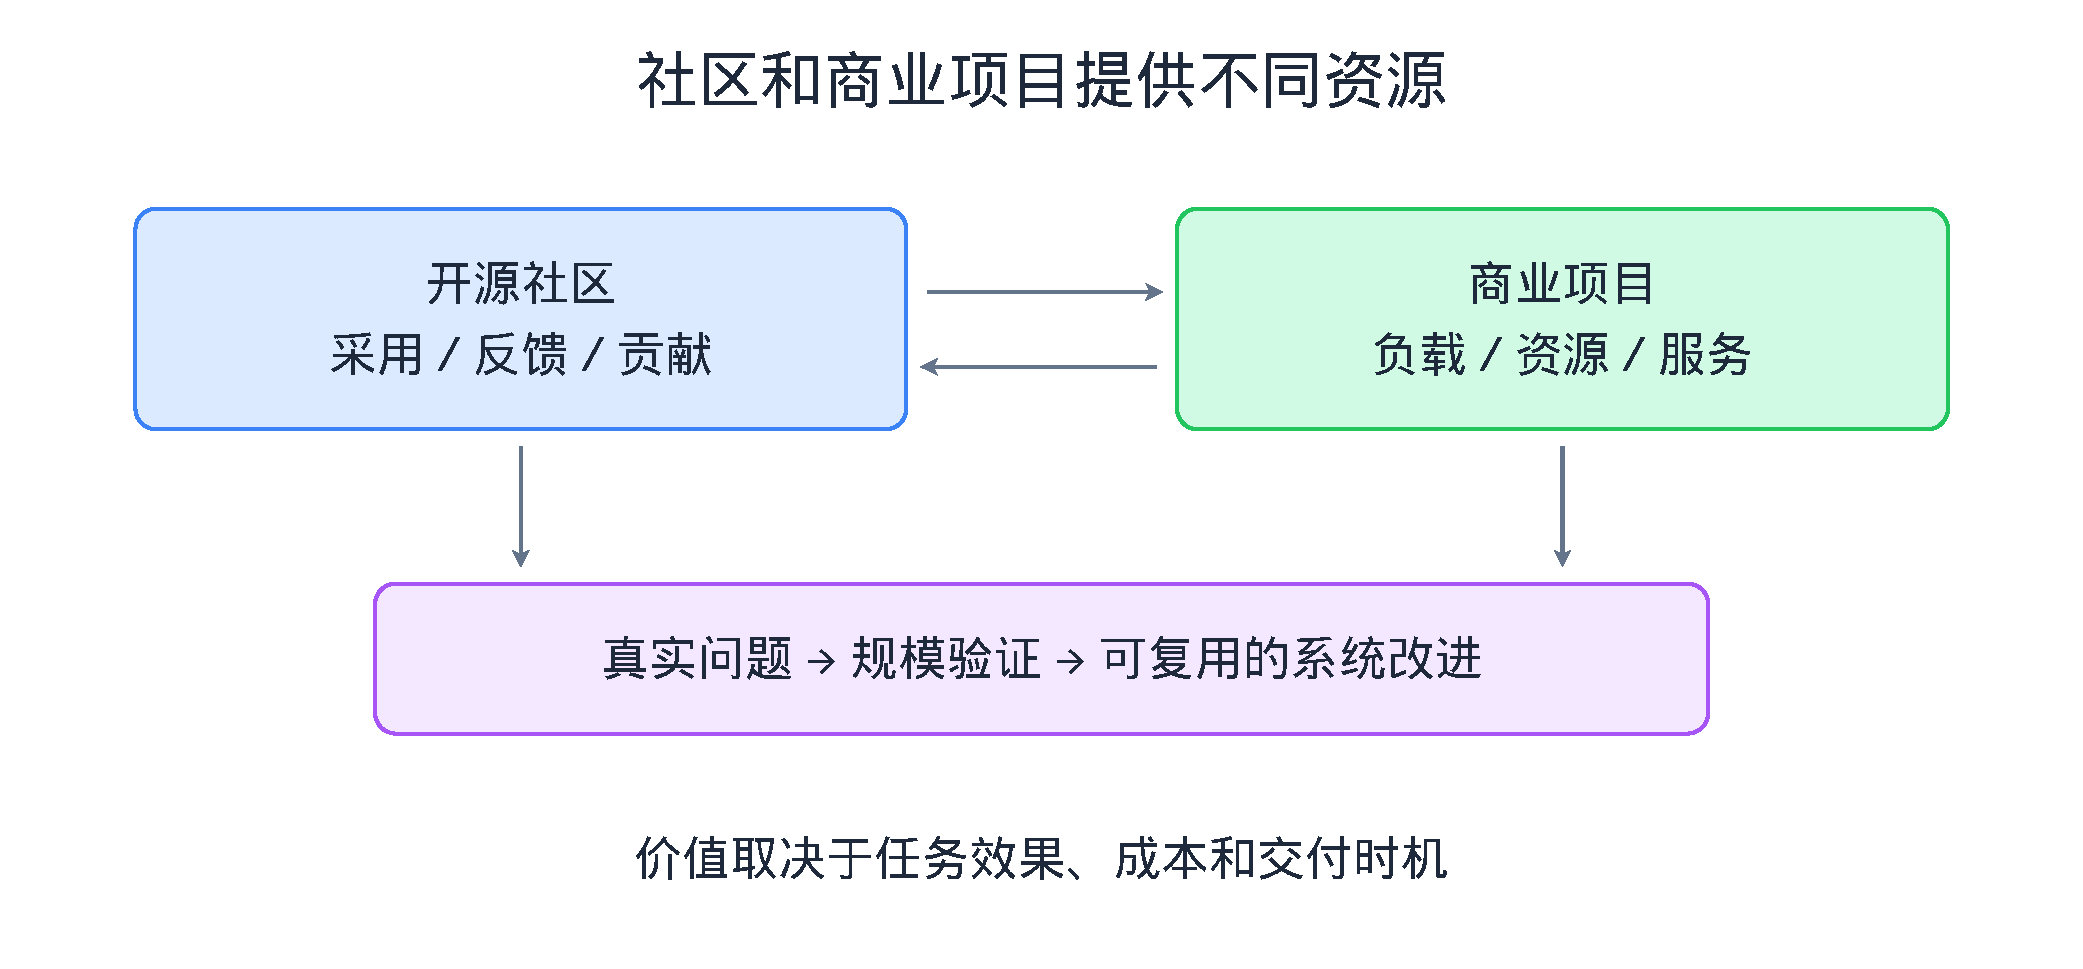
\includegraphics[width=\linewidth,height=.68\textheight,keepaspectratio]{assets/open-commercial.pdf}
\caption{社区和商业项目提供不同资源；依据节目口述整理（00:39:45–00:40:32；01:12:32–01:14:12）}
\end{figure}
\begin{knowledgebox}{读图：开源社区怎样连接研究与创业}
图上方左右并列两个方框：左侧为“开源社区（采用／反馈／贡献）”，右侧为“商业项目（负载／资源／服务）”，二者之间有两条方向相反的水平箭头，表示双向互动。左右两个方框底部各有一条向下箭头，共同指向中间的横框“真实问题 \ensuremath{\rightarrow} 规模验证 \ensuremath{\rightarrow} 可复用的系统改进”。图最下方一行文字总结了用户与市场衡量系统的基础：“价值取决于任务效果、成本和交付时机”。
\end{knowledgebox}
由此可见，开源社区带来广泛采用与问题反馈，商业项目提供真实工作负载与大规模算力资源，二者共同促成经过规模验证的系统改进。下一章将进一步探讨智能体落地后的评测标准与工程师个人角色的变化。
\needspace{6\baselineskip}\subsection{本章小结}
\begin{enumerate}
\item 技术创业需关注市场时机：2023 年不少客户将具备多轮工具调用能力的智能体与仅做信息检索补充的 RAG 混淆，过早切入需要承担较高的市场教育成本。
\item 开源社区与商业项目可以相互支持：商业合作提供的算力与负载能帮助开源框架完成千卡级规模验证；而针对极端场景的优化因普通用户极少用到，对社区帮助有限，未必全部开源。
\item 从具体系统工具走向平台愿景：在扎实做好 SGLang 推理与 Miles 后训练框架的基础上，团队希望探索支持多元智能体互联与人机交互接口的开放平台可能性。
\end{enumerate}
\needspace{8\baselineskip}\section{Agent 时代的评测、技术品味与职业选择}
前一章梳理了开源社区与商业基础设施如何协同演化。当底层系统把智能体带入日常研发与各行各业后，衡量模型好坏的标尺、软件工程的组织形态以及个人的职业选择都随之改变。本章结合朱邦华在访谈尾声的思考，解析评测体系如何从人类偏好转向任务验证、编程智能体如何重塑工程分工，以及在技术快速迭代期如何锤炼技术品味并做出理性的路径取舍。
\needspace{6\baselineskip}\subsection{喜欢一个回答与完成一个任务}
在评估大语言模型时，首先需要区分“人类主观喜欢一个回答”与“模型客观完成一项复杂任务”。在 01:29:27–01:31:14 讨论 LM Arena（早期称为 Chatbot Arena，一种让两个匿名模型针对同一提示词生成回答、由人类用户盲测投票并按竞技积分规则计算排名的众包评测平台）获得高额融资时，朱邦华指出，早期版本之所以备受关注，是因为当时的模型尚难稳定输出高质量内容，评测的核心诉求是检验聊天体验是否自然、语气是否讨人喜欢。

为什么仅靠人类即时偏好的投票不足以覆盖前沿需求？随着模型研发向智能边界（Intelligence Frontier）推进，研究与工业界越来越关注模型能否解决复杂的工程与编程等高难度问题。虽然人类评审也可以具备专业知识，但在常规众包盲测的交互形式下，单靠对回答的直观喜好很难直接检验一段复杂代码或深层推理是否真正解决了问题。

因此，推进智能边界的评测需要与可验证奖励强化学习（RLVR）的思路相呼应，在偏好评测之外补充可交互、可验证的任务环境。例如在编程任务中，通过检验代码能否正确运行并达成目标来客观评估模型能否解决问题。偏好评测与客观任务验证分别回答了“回答是否讨喜自然”与“复杂任务是否真正完成”这两个互补的问题，朱邦华也认为评测平台未来需要向复杂任务验证方向拓展。

\needspace{6\baselineskip}\subsection{Coding Agent 放大了什么能力}
当模型解决复杂任务的能力落地为 Claude Code 等编程智能体（Coding Agent，能够读取代码库、编写修改代码并配合终端工具迭代任务的 AI 系统）时，软件工程行业的分工可能发生怎样的变化？在 01:31:17–01:35:32 的交流中，朱邦华分享了他对计算机行业就业趋势的个人构想：编程智能体给不同阶段的开发者带来了两方面影响。

一方面，对于初级软件工程师（Junior Software Engineer）或刚毕业的计算机科学（Computer Science, CS）学生而言，求职可能会变得更难，因为一些较为基础的计算机与软件工程工作更容易由智能体承担；另一方面，资源可能会进一步向有技术品味（Taste）、高水平的系统工程师、软件工程师和研究员集中，因为智能体能够放大他们的能力并加快迭代速度（Iteration Speed）。朱邦华推想，过去维护一个复杂软件系统可能需要上百人甚至上千人的团队，而随着编程智能体不断变强，未来在智能体原生的组织方式下，也许十几个很强、很有品味的系统工程师借助智能体就能把同等复杂度的系统做起来。

这种变化也引出了他坦言自己尚未想清楚的难题：如果初级岗位需求减少，学校培养与顶尖系统工程师之间的教育断层该如何弥补？同时他也提到，在假设人工智能仍需进一步发展的情况下，一部分人力需求可能会转向门槛越来越高、需要密集人力资本投入的复杂数据标注（Data Labeling，已不再是简单的偏好对比，而是构造高难度训练数据）；而对于非计算机专业的人士（例如计算生物学等领域的研究者），人工智能工具则降低了编程与跨界进入新方向的门槛，使更多人能借助工具去做自己真正感兴趣的事。当然，他也指出社会转型过程不可避免会给部分从业者带来现实的求职阵痛。

\needspace{6\baselineskip}\subsection{把技术品味落实到改进方案}
既然编程智能体能放大工程师的能力，那么在招聘与日常自我提升中，究竟该如何定义和识别所谓的“技术品味（Taste）”？在 01:39:04–01:44:17 的探讨中，嘉宾强调，技术品味在工程实践中最直观的体现，是对代码与系统设计抱有强烈的批判性思维（Criticism）与质量把关（Gatekeeping，在代码合入主干前审查架构合理性与简洁度、拒绝低质量实现的工程机制）意识。

在面试或日常交流中，有些开发者面对现有代码会觉得“还不错、能用就行”并直接接受；而有品味的工程师看到结构不佳的代码会感到不自在，希望动手重写和改进。朱邦华借用 Linux 内核社区的开发方式作比喻：核心维护者把提交代码的贡献者当作执行者，对代码质量做严格把关，不符合设计审美的代码就会被拒绝。放到今天与编程智能体的协作中（这里借用的是严格把控代码质量的机制，而非鼓励网络攻击或辱骂），如果一名开发者觉得智能体写出的代码已经很好、无需挑剔，那么他的产出表现就容易停留在智能体的默认水平；只有当开发者能够识别出现有代码到底哪里有问题，并且能告诉智能体真正高质量的代码应该长什么样、给出更好的解决方案时，才能驱动智能体写出高质量的代码。

这种对代码质量的执着在大公司里有时会被视为“难合作”或“阻碍进度”，但在 LMSYS 和 RadixArk 的团队文化中，他们恰恰希望发掘并支持这类精益求精的人。同时，朱邦华与主持人都强调，在技术能力与品味之外，寻找创业伙伴与团队成员最重要的底线是“正直善良”的人格底色。只有建立在真诚、可靠的基础上，严格的工程探讨才能转化为团队的共同进步。

\needspace{6\baselineskip}\subsection{保持探索，也学会放下旧路径}
面对技术范式与就业环境的剧烈变化，处于本科、博士或职场不同阶段的年轻人该如何做出自己的道路选择？在访谈最后的建议环节，朱邦华结合自身从通信工程、计算生物学到统计与强化学习理论，最终在博士第五年转向大模型与基础设施的经历，分享了一条核心的实践经验：在高速变化的时代，敢于探索新方向，并学会适时放下已有的沉没成本。

在他看来，当技术处于快速变化的阶段时，试错成本有时比人们担心的要低：只要顺着技术发展的大方向去探索，主动放下过去积累的部分经验或标签，往往能接触到新的机会并获得成长。许多人在考虑是否转向新方向或尝试创业公司项目时犹豫不决，常常是受制于已有的路径依赖。

结合前文与本节的讨论，不同阶段的读者可以根据自身处境具体权衡：对于刚读博士的同学，不必因为前两三年还没有亮眼成果而过度焦虑，可以在持续探索中寻找真正有影响力的突破口；对于正在纠结去向或已在工作的同学，如果有自己特别想尝试的方向，或者遇到了资源充足、能接触前沿技术的机会，当心里产生“为什么别人能做而我就做不了”的想法时，不妨结合自身条件亲自去试一试。

\begin{importantbox}{如何通过代码审查与改进方案驱动 Coding Agent}
在使用 Claude Code 等编程智能体时，工程判断力如何影响最终的代码质量？
\begin{enumerate}
\item 被动接受默认输出：如果开发者对代码结构缺乏挑剔意识，觉得生成的代码“能跑就行”，就容易放过冗余实现与设计隐患，产出质量停留在智能体的默认水平。
\item 识别问题并给出方案：有技术品味的工程师在审查代码时，不仅能判断“这段代码写得不够好”，还能准确定位它到底存在什么问题，并提出更简洁、合理的改进方案。通过“严格把关（Gatekeeping）—指出具体问题—提供改进方向”的循环，开发者能够驱动智能体写出更高质量的系统代码。
\end{enumerate}
\end{importantbox}
\begin{warningbox}{选择下一步方向时可以检查哪些条件}
在决定是否转换研究课题、加入初创团队或在学业与工业界之间做取舍时，可以依次检查以下四个实际条件：
\begin{enumerate}
\item 个人兴趣与动力：自己是否真正对目标方向感到好奇，而非仅仅跟风短期热点？
\item 想要解决的问题：目标方向是在解决真实世界中的关键瓶颈，还是边际收益递减的旧问题？
\item 训练环境与资源：目标平台能否提供解决问题所需的算力、数据或智能体工具额度，帮助自己积累一线经验？
\item 个人处境与责任：在放下旧路径的沉没成本时，当前的学业阶段、工作状态与家庭支持条件是否允许承担相应的试错风险？
\end{enumerate}
\end{warningbox}
\begin{table}[H]\centering\small
\caption{Agent 时代的评测方式、工程分工与个人能力要求对比}
\begin{tabular}{>{\raggedright\arraybackslash}p{\dimexpr(\linewidth-6\tabcolsep)/3\relax}>{\raggedright\arraybackslash}p{\dimexpr(\linewidth-6\tabcolsep)/3\relax}>{\raggedright\arraybackslash}p{\dimexpr(\linewidth-6\tabcolsep)/3\relax}}
\toprule
维度 & 解决的核心问题 & 机制特征与实践关系\\\midrule
众包偏好评测 (如早期 LM Arena) & 衡量模型对话的自然度与人类主观喜爱程度 & 依赖盲测对比投票；反映对话体验偏好，但与复杂编程和任务完成的客观验证侧重点不同\\[4pt]
智能边界与任务验证评测 & 检验模型能否真正解决复杂的端到端工程与推理问题 & 构建可执行环境与客观验证指标；从“回答讨喜”转向“任务真正跑通”\\[4pt]
编程智能体 (Coding Agent) 协作 & 承担基础编码环节，放大系统工程师的迭代速度并降低跨界编程门槛 & 据嘉宾分析，这可能增加初级岗位求职难度、促使资源向高水平工程师集中，同时赋能非 CS 领域研究者\\[4pt]
技术品味与代码把关 (Gatekeeping) & 避免被动接受低质量代码，提高人机协作的产出质量 & 要求工程师不仅能对坏代码产生不适，还能准确定位问题并给出优雅的架构改进方案\\[4pt]
\bottomrule\end{tabular}\end{table}
随着模型评测从对话偏好走向复杂任务验证，以及编程智能体进入日常软件开发，工程师的角色越来越聚焦于定义标准、检验结果与指导改进。下图展示了人的技术判断如何驱动智能体产出高质量结果。
\begin{figure}[H]\centering
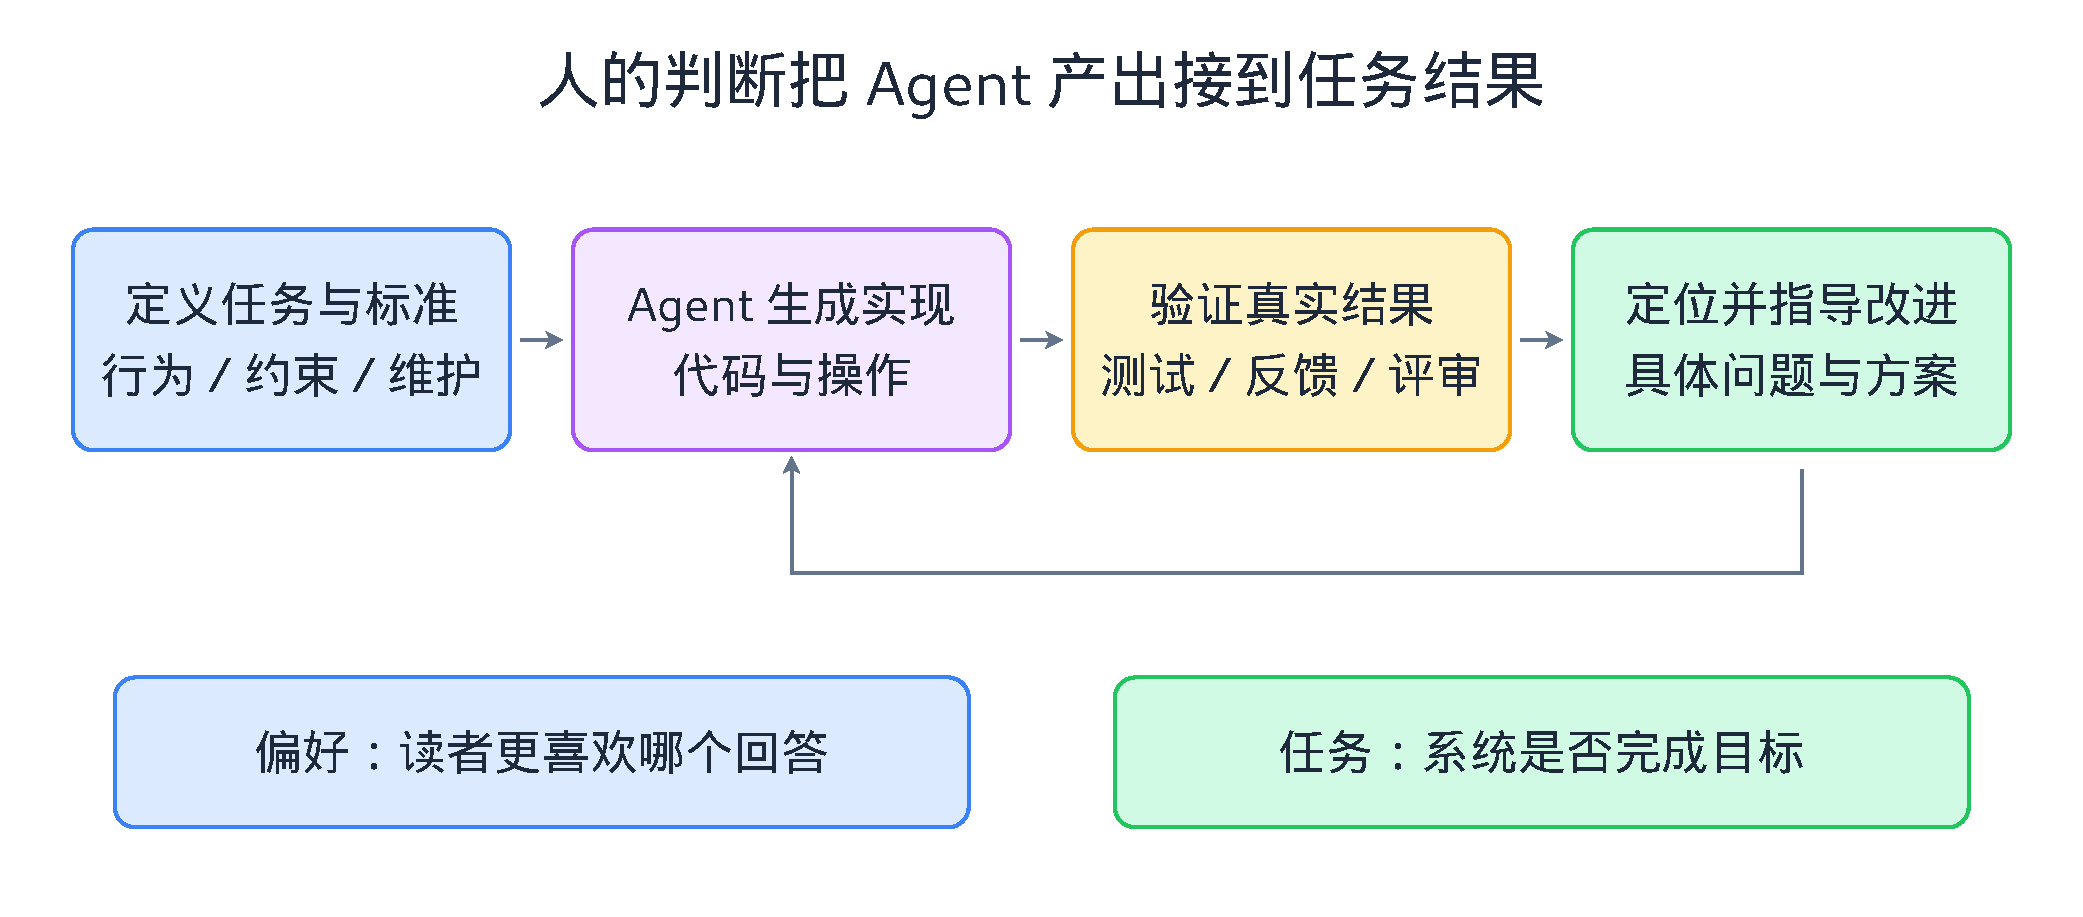
\includegraphics[width=\linewidth,height=.68\textheight,keepaspectratio]{assets/agent-quality-loop.pdf}
\caption{人的判断把 Agent 产出接到任务结果；依据节目口述整理（01:29:27–01:46:09）}
\end{figure}
\begin{knowledgebox}{读图：Agent 时代的评测、技术品味与职业选择}
图上方由四个从左到右依次以箭头相连的方框组成：“定义任务与标准（行为／约束／维护）”指向“Agent 生成实现（代码与操作）”，再指向“验证真实结果（测试／反馈／评审）”，最后指向“定位并指导改进（具体问题与方案）”。一条回流箭头从最右侧“定位并指导改进”底部引出，指回第二个方框“Agent 生成实现”，形成迭代改进闭环。图下方左右并列两个方框，分别标注“偏好：读者更喜欢哪个回答”与“任务：系统是否完成目标”。
\end{knowledgebox}
该图总结了本章的核心论点：偏好评测与任务验证回答的是不同维度的问题；而在工程协作中，只有当开发者能够依据维护标准验证结果、准确定位缺陷并给出方案时，智能体的生成能力才能转化为可靠的系统成果。
\needspace{6\baselineskip}\subsection{本章小结}
\begin{enumerate}
\item 偏好评测与任务验证相互补充：早期盲测榜单主要反映聊天回答是否受人喜爱，而推进智能边界还需要构建可验证环境来检验复杂编程与问题解决能力。
\item 编程智能体正在改变工程协作与跨界门槛：据朱邦华分析，基础编码环节更容易由智能体承担，而具备系统品味的核心工程师则能借助智能体加快迭代速度，非计算机专业人员也能借此降低使用代码的门槛。
\item 技术品味、正直底色与适时取舍同样重要：工程品味体现在能定位代码问题并给出改进方案；团队合作需以正直善良为底色；在面对新机会时，结合自身兴趣与资源条件学会放下旧路径的沉没成本，有助于在变革期把握方向。
\end{enumerate}
\needspace{8\baselineskip}\section{总结与延伸}
纵观全书，大模型基础设施的演进始终围绕着“如何以更高效率将算力与反馈转化为解决复杂任务的能力”这一主线。从单机推理到千卡、万卡级别的强化学习训练，技术重心正从静态文本生成转向包含工具调用、代码执行与多模态交互的动态闭环。在这一过程中，底层系统的可靠性、环境执行的并发与时延控制、奖励机制的精细设计，共同决定了模型后训练能否走通。

结合朱邦华在访谈尾声的分享，面对技术范式的快速更替，无论处于求学还是职场阶段，都需要在拓宽视野的同时学会放下旧路径的沉没成本。但这并非提倡盲目跟风，而是建立在对问题约束、个人兴趣与平台资源的审慎评估之上。为把书中的机制理解转化为实际能力，读者可以遵循以下三条可操作的学习与实践路径：

第一，动手跑通推理与后训练的基础链路。从部署 SGLang 等开源推理引擎入手，观察前缀缓存与批处理对吞吐量的影响；再结合小型开源权重，尝试用 PPO 完成一轮后训练实验，观察价值网络损失与策略更新；再比较 DPO 或 GRPO 如何省去独立的价值网络。

第二，关注可执行环境与系统瓶颈。在构建智能体应用时，不仅关注提示词设计，还要实际测量函数调用、容器沙箱启动和外部工具执行的时延与并发表现，训练从全链路排查瓶颈的系统视角。

第三，在日常使用编程智能体时锤炼代码把关能力。拒绝“能跑就行”的被动接受心态，每次审查生成代码时主动定位冗余结构、接口缺陷或边界隐患，并练习向智能体给出清晰、可验证的重构方案，在人机协作中持续提升工程品味。
\subsection{拓展阅读}
以下资料供回看节目、查阅术语与继续学习。
\begin{itemize}
\item 月球大叔：本期完整视频：\url{https://www.youtube.com/watch?v=VoAaX02cHFE}
\item 官方完整逐字稿：\url{https://unclemoon.ai/blog/001-zhu-banghua/transcript/}
\item 官方访谈文章：\url{https://unclemoon.ai/blog/001-zhu-banghua/}
\item SGLang 官方项目：\url{https://github.com/sgl-project/sglang}
\item DeepSeek-R1 官方报告与模型说明：\url{https://github.com/deepseek-ai/DeepSeek-R1}
\end{itemize}
\end{document}
